%------------------------------------------------------%
% B.Tech CSE (CYS) Project Latex Template
%
% Authors: Dr. Lakshmy K V and Ramaguru Radhakrishnan
% Date   : 10 - APR - 2025
%------------------------------------------------------%
\documentclass[12pt,a4paper]{report}

\usepackage[margin=1in]{geometry}
\usepackage [english]{babel} % Sets document language to English for proper hyphenation and typographic rules.
\usepackage [autostyle, english = american]{csquotes} % For smart quotation marks and language-specific quoting styles.


\usepackage{bold-extra} % Allows use of \textbold for bold small caps and other font enhancements.
\usepackage{amsmath} % Provides advanced math environments and symbols.
\usepackage{amsfonts}  % Gives access to additional math fonts like \mathbb and \mathfrak.
\usepackage{amssymb}  % Provides additional mathematical symbols.
\usepackage{amsthm} % Provides theorem-like environments (e.g., theorems, definitions).
\theoremstyle{definition} % Sets the style for theorem environments (like definitions) to non-italic.
\usepackage{float}  % Provides H placement specifier for figures and tables.
\newtheorem{Definition}{Definition}[section] % Defines a new theorem-like environment for definitions, numbered by section.

\MakeOuterQuote{"}  % Makes double quotes act as smart quotes automatically.
\usepackage{setspace}  % Allows setting of line spacing, such as \onehalfspacing.
\onehalfspacing  % Sets 1.5 line spacing throughout the document for readability.

\usepackage{graphicx} % Used for including images and graphics with \includegraphics.
\graphicspath{{Figures/}} % Sets the default directory for images to "Figures/".

\usepackage{array}  % Enhances table formatting, e.g., custom column types.
\usepackage{soul} % highlighting 

\usepackage{cite} % Improves citation handling and compresses numerical citation ranges.

\usepackage{natbib}  % Provides flexible citation styles (author-year and numeric).

\usepackage{longtable} % Allows tables to span multiple pages.

\usepackage{fancyhdr}  % For customizing headers and footers.
\usepackage{titletoc} % Customizes table of contents formatting.

\usepackage{tabto}  % Enables tabbing at specific horizontal positions.
\usepackage{enumitem} % Allows customization of list environments (e.g., spacing, labels).
\newcolumntype{P}[1]{>{\centering\arraybackslash}p{#1}} % Defines a new centered column type for tables.

\setcitestyle{square} % Sets citation style to use square brackets (e.g., [1], [2]).

\usepackage{algorithm} % Used to create floating algorithm environments; useful for inserting algorithms with captions and labels.
% Alternatively, \usepackage[ruled,vlined]{algorithm2e} % An alternative algorithm package that offers more styling options (rules, lines, etc.)
\usepackage{algpseudocode} % Provides the 'algorithmic' environment for writing pseudocode in combination with 'algorithm'.

\usepackage{xcolor} % Adds color support to LaTeX (for text, tables, links, etc.), extends the basic color capabilities.
\definecolor{darkgray}{rgb}{0.4, 0.4, 0.4} % Defines a custom color named 'darkgray' using RGB values.

\usepackage{hyperref} % Enables hyperlinks within the document and to external URLs.
\hypersetup{
	colorlinks=true, % Enables colored links instead of boxed links.
	linkcolor=blue, % Color of internal document links (e.g., table of contents).
	filecolor=blue,  % Color for file links (e.g., PDF attachments).   
	urlcolor=blue,  % Color for hyperlinks (URLs).
	citecolor=blue  % Color for citation links.
}

%-----------------------------------------------------%
%              Code Listing Settings
%-----------------------------------------------------%
\usepackage{listings} % Used to display source code listings with syntax highlighting, line numbers, etc.

\lstdefinelanguage{Python}{
    keywords={def, return, if, elif, else, while, for, break, continue, pass, import, from, as, class, try, except, finally, raise, with, lambda, assert, yield, global, nonlocal, True, False, None, and, or, not, in, is},
    keywordstyle=\color{blue}\bfseries,
    ndkeywords={self, cls, __init__, __name__, __main__, print, input, range, len, list, dict, tuple, set, str, int, float, bool, open, read, write, close, map, filter, zip, enumerate},
    ndkeywordstyle=\color{darkgray}\bfseries,
    identifierstyle=\color{black},
    sensitive=true,
    comment=[l]{\#},
    morecomment=[s]{"""}{"""},
    morecomment=[s]{'''}{'''},
    commentstyle=\color{magenta}\ttfamily,
    stringstyle=\color{red}\ttfamily,
    morestring=[b]',
    morestring=[b]"
}

\newcommand{\CodeStyle}{
	\lstset{ 
        numbers=left,                   
        stepnumber=1,                   
        numbersep=5pt,                   
        showspaces=false,               
        showstringspaces=false,         
        showtabs=false,                 
        frame=single,                          
        tabsize=2,                      
        captionpos=b,                   
        breaklines=true,                
        breakatwhitespace=false,
        keywordstyle=\textcolor{blue},
        commentstyle=\color{magenta},
        stringstyle=\color{red},
    }
}

%-----------------------------------------------------%
%              Project Specific Section
%-----------------------------------------------------%

\newcommand{\topic}{Quantum Secure File Transfer Protocol}
\newcommand{\SOneName}{Arul Sujith S}
\newcommand{\SOneRN}{CB.EN.U4CYS22008}
\newcommand{\STwoName}{Hemadhri P C}
\newcommand{\STwoRN}{CB.EN.U4CYS22026}
\newcommand{\SThreeName}{J.P. Hemanth Kumaar}
\newcommand{\SThreeRN}{CB.EN.U4CYS22028}
\newcommand{\SFourName}{Jose Rohit M}
\newcommand{\SFourRN}{CB.EN.U4CYS22030}
\newcommand{\gname}{Dr. Aravind Vishnu S S} % Guide Name
\newcommand{\gdes}{Assistant Professor } % Guide Designation
\newcommand{\dept}{TIFAC-CORE IN CYBER SECURITY}
\newcommand{\spec}{Computer Science And Engineering (Cyber Security)}
\newcommand{\yearofpassing}{NOVEMBER 2025} %Project Graduation


%-----------------------------------------------------%
%              Start of Document
%-----------------------------------------------------%

% Document Start
\begin{document}
%-----------------------------------------------------%
%                 Title Page
%-----------------------------------------------------%
	\begin{titlepage}
    \begin{center}
        \Large
        \textbf{\topic}
        
        \vspace*{32pt}
        \normalsize
        PROJECT REPORT 
        
        \vspace*{32pt}
        \textbf{\textit{Submitted by}}
        
        \vspace*{24pt}
        \begin{tabular}{@{} l l @{}}
            \SOneName   & \SOneRN   \\
            \STwoName   & \STwoRN   \\
            \SThreeName & \SThreeRN \\
            \SFourName  & \SFourRN  \\
        \end{tabular}
        
        \vspace*{32pt}
        \normalsize
        \textit{\textbf{in partial fulfillment for the award of the degree}}
        
        \vspace*{10pt}
        \textbf{\textit{of}}
        
        \vspace*{10pt}
        \textbf{Bachelor of Technology}
        
        \vspace*{10pt}
        in
        
        \vspace*{10pt}
        \textbf{\spec}
        
        \vspace*{32pt}
        
\includegraphics[scale=0.7]{Logo1.jpg}
        
        \vspace*{20pt}
        \normalsize
        \textbf{\dept}
        
        \vspace*{5pt}
        AMRITA SCHOOL OF COMPUTING
        
        \vspace*{5pt}
        \large
        \textbf{AMRITA VISHWA VIDYAPEETHAM}
        
        \vspace*{5pt}
        \normalsize
        COIMBATORE - 641 112
        
        \vspace*{10pt}
        \yearofpassing
    \end{center}
\end{titlepage}

%-----------------------------------------------------%
%               Bonafide certificate
%-----------------------------------------------------%

\clearpage
\thispagestyle{empty}
\begin{titlepage}
    \begin{center}
        \Large
        \textbf{\topic}
        
        \vspace*{15pt}
        \normalsize
        PROJECT REPORT 
        
        \vspace*{15pt}
        \textbf{\textit{Submitted by}}
        
        \vspace*{15pt}
        \begin{tabular}{@{} l l @{}}
            \SOneName   & \SOneRN   \\
            \STwoName   & \STwoRN   \\
            \SThreeName & \SThreeRN \\
            \SFourName  & \SFourRN  \\
        \end{tabular}
        
        \vspace*{18pt}
        \normalsize
        \textit{\textbf{in partial fulfillment for the award of the degree}}
        
        \vspace*{8pt}
        \textbf{\textit{of}}
        
        \vspace*{8pt}
        \textbf{Bachelor of Technology}
        
        \vspace*{8pt}
        in
        
        \vspace*{8pt}
        \textbf{\spec}
        
        \vspace*{18pt}
        \textit{Under the guidance of}
        
        \vspace*{8pt}
        {\bfseries \gname} \\
        \gdes \\
        Amrita Vishwa Vidyapeetham \\
        Coimbatore
        
        \vspace*{18pt}
        
\includegraphics[scale=0.7]{Logo1.jpg}
        
        \vspace*{10pt}
        \normalsize
        \textbf{\dept}
        
        \vspace*{5pt}
        AMRITA SCHOOL OF COMPUTING
        
        \vspace*{5pt}
        \large
        \textbf{AMRITA VISHWA VIDYAPEETHAM}
        
        \vspace*{5pt}
        \normalsize
        COIMBATORE - 641 112
        
        \vspace*{10pt}
        \yearofpassing
    \end{center}
\end{titlepage}
    	
%-----------------------------------------------------%
%               Bonafide certificate
%-----------------------------------------------------%
	\clearpage
\thispagestyle{empty}
\newpage

\begin{center}
    {\Large \textbf{AMRITA VISHWA VIDYAPEETHAM}}\\[5pt]
    {\large \textbf{AMRITA SCHOOL OF COMPUTING}}\\
    {\large \textbf{COIMBATORE - 641 112}}\\[1cm]
    
    
\includegraphics[scale=0.70]{Figures/Logo1.jpg}\\[1cm]
    
    {\large \textbf{BONAFIDE CERTIFICATE}}
\end{center}

\vspace{0.5cm}

\noindent This is to certify that this project entitled \textbf{"\topic"} submitted by 
\textbf{\SOneName\ (\SOneRN), 
\STwoName\ (\STwoRN), 
\SThreeName\ (\SThreeRN), 
\SFourName\ (\SFourRN)}, in partial fulfillment of the requirements for the award of the \textbf{Degree of Bachelor of Technology} in \textbf{\spec} is a bonafide record of the work carried out by them under my guidance and supervision at Amrita School of Computing, Coimbatore.

\vspace{1.5cm}

\noindent\begin{minipage}[t]{0.48\textwidth}
\textbf{\gname} \\
\gdes
\end{minipage}%
\hfill
\begin{minipage}[t]{0.48\textwidth}
\raggedleft
\textbf{Prof. M. Sethumadhavan} \\
Professor and Head
\end{minipage}

\vspace{2cm}

\noindent This project report was evaluated by us on \underline{\hspace{5cm}}.

\vspace{4cm}

\noindent\begin{minipage}[t]{0.48\textwidth}
\textbf{INTERNAL EXAMINER}
\end{minipage}%
\hfill
\begin{minipage}[t]{0.48\textwidth}
\raggedleft
\textbf{EXTERNAL EXAMINER}
\end{minipage}

	
%-----------------------------------------------------%
%                Declaration Page
%-----------------------------------------------------%
	
\begin{titlepage}
    \begin{center}
        \large
        \textbf{AMRITA VISHWA VIDYAPEETHAM}\\[5pt]
        \normalsize
        \textbf{AMRITA SCHOOL OF COMPUTING, COIMBATORE}\\[3pt]
        \textbf{TIFAC-CORE IN CYBER SECURITY}\\[32pt]

        \normalsize
        \textbf{DECLARATION}
    \end{center}

    \vspace{22pt}

    \begin{sloppypar}
    \noindent
    We hereby declare that this project entitled \textbf{``\topic''} is a record of the original work done by us under the guidance of \textbf{\gname}, \gdes, TIFAC-CORE in Cyber Security, Amrita Vishwa Vidyapeetham and that this work has not formed the basis for the award of any degree, diploma, associateship, fellowship, or any other similar title, to any candidate in any university, to the best of our knowledge.
    \end{sloppypar}

    \vspace{25pt}

    \noindent\textbf{Place:} Coimbatore \hfill \textbf{Date:} \underline{\hspace{4cm}}

    \vspace{1.2cm}

    \noindent
    \vspace{0.5cm}\SOneName\ (\SOneRN)\\[8pt]  
    \vspace{0.5cm}\STwoName\ (\STwoRN)\\[8pt] 
    \vspace{0.5cm}\SThreeName\ (\SThreeRN)\\[8pt] 
    \vspace{0.5cm}\SFourName\ (\SFourRN)\\[8pt] 


    \vfill

    \begin{center}
        \textbf{COUNTERSIGNED}\\[50pt]
        \textbf{Prof. M. Sethumadhavan}\\
        Professor and Head,\\
        TIFAC-CORE in Cyber Security
    \end{center}

\end{titlepage}

\clearpage
	
%-----------------------------------------------------%
%             Acknowledgements
%-----------------------------------------------------%
    
	\begin{titlepage}
    \begin{center}
        \huge{\textbf{Acknowledgment}}
    \end{center}
    
    \normalsize
    \vspace*{22pt}
    \begin{sloppypar}
        \noindent
        \baselineskip 0.7 cm
        At the very outset, we would like to offer our heartfelt gratitude to the \textbf{Almighty}, whose blessings gave us the strength, wisdom, and perseverance to complete this project.
        
        \vspace*{12pt}
        \noindent
        We express our sincere thanks to our guide, \textbf{\gname}, \gdes, TIFAC-CORE in Cyber Security, Amrita Vishwa Vidyapeetham, for his valuable guidance, continuous encouragement, and technical insights throughout the project.
        
        \vspace*{12pt}
        \noindent
        We are immensely grateful to \textbf{Prof. M. Sethumadhavan}, Professor and Head, TIFAC-CORE in Cyber Security, for his visionary leadership.
        
        \vspace*{12pt}
        \noindent
        We would also like to extend our heartfelt thanks to \textbf{Mr. Sitaram Chamarty}, Professor of Practice, TIFAC-CORE in Cyber Security, Amrita Vishwa Vidyapeetham, for his constructive feedback, mentoring, expert knowledge shared during key phases of development.
        
        \vspace*{12pt}
        \noindent
        We wish to acknowledge the contributions of our family, friends, and seniors for their constant encouragement, emotional support, and constructive discussions. Their curiosity and questions helped us view our work from new perspectives and strengthened our understanding of the subject.
        
        \vspace*{12pt}
        \noindent
        We are also thankful to all the faculty members of TIFAC-CORE in Cyber Security, whose direct or indirect support and encouragement played a vital role in the successful completion of this project.
        

    \end{sloppypar}
\end{titlepage}

    
%-----------------------------------------------------%
%               Project Abstract
%-----------------------------------------------------%
	
\clearpage 	
\pagenumbering{roman}
\section*{{\centerline{\huge Abstract}}\hfill} \addcontentsline{toc}{chapter}{Abstract}
\vspace*{22pt}
\baselineskip 0.7 cm 

The rapid advancement of quantum computing poses an existential threat to classical cryptographic systems that underpin secure communication protocols. Shor's algorithm enables quantum computers to break RSA and Elliptic Curve Cryptography in polynomial time, rendering current Secure File Transfer Protocols (SFTP) fundamentally insecure. The ``Harvest Now, Decrypt Later'' (HNDL) threat model further demands proactive migration to quantum-resistant alternatives.

This project presents the design and implementation of a \textbf{Quantum Secure File Transfer Protocol (Q-SFTP)}, a production-grade, post-quantum variant of SFTP that replaces vulnerable classical algorithms with NIST-standardized post-quantum cryptographic (PQC) primitives: \textbf{CRYSTALS-Kyber512} (ML-KEM, FIPS 203) for key encapsulation and \textbf{CRYSTALS-Dilithium2} (ML-DSA, FIPS 204) for digital signatures, combined with AES-256-GCM for symmetric encryption and BLAKE2b-256 for file integrity verification.

Q-SFTP introduces a novel four-phase mutual authentication handshake protocol, role-based access control (RBAC) with per-user directory isolation, automatic metadata stripping (EXIF, PDF, DOCX) for privacy preservation, malicious file protection via extension blacklisting and magic number validation, a chunked resumable transfer mechanism with persistent state tracking, and a comprehensive activity logging system with IP anonymization. The system is deployed as a modern web application with a browser-based GUI that abstracts all cryptographic complexity behind an intuitive FTP-style interface, including an admin panel for user and system management.

Experimental evaluations confirm that Q-SFTP provides resistance to quantum cryptanalysis, man-in-the-middle attacks, replay attacks, and data tampering, while maintaining acceptable performance characteristics with approximately 0.01\% cryptographic overhead per file transfer.

\vspace*{12pt}
\noindent \textbf{Keywords:} Post-Quantum Cryptography, CRYSTALS-Kyber, CRYSTALS-Dilithium, Secure File Transfer, BLAKE2b, AES-256-GCM, Resumable Transfers, Role-Based Access Control, Metadata Stripping, Docker, Flask



%-----------------------------------------------------%
%               Table of Contents
%-----------------------------------------------------%  
	\clearpage
\pagenumbering{roman}

% Table of Contents
\renewcommand*\contentsname{Table of Contents}
\tableofcontents

% List of Figures
\clearpage
\addcontentsline{toc}{chapter}{List of Figures}
\listoffigures

% List of Algorithms
\clearpage
\addcontentsline{toc}{chapter}{List of Algorithms}
\listofalgorithms

% Start of main content
\clearpage
\pagestyle{fancy}
\fancyhf{}
\rhead{\thepage}
\lhead{}
\pagenumbering{arabic}
\setcounter{page}{1}

%-----------------------------------------------------%
%               Chapters
%-----------------------------------------------------%
\chapter{Introduction} 
\lhead{Chapter 1. \emph{Introduction}}
\label{chap.1}

\section{Motivation}

The widespread deployment of quantum computing threatens the security of current encryption systems that protect file transfer protocols. Shor's algorithm, when executed on a sufficiently powerful quantum computer, can factor large integers and compute discrete logarithms in polynomial time — breaking RSA, DSA, and Elliptic-Curve Diffie-Hellman (ECDH) \cite{shor1994algorithms}. Grover's algorithm provides a quadratic speedup for symmetric key search, effectively halving the security level of symmetric ciphers \cite{grover1996fast}.

Of particular concern is the \textit{``Harvest Now, Decrypt Later''} (HNDL) threat model, where adversaries capture encrypted network traffic today for decryption once quantum computers become available \cite{mosca2018cybersecurity}. This threat demands proactive migration to quantum-resistant alternatives, especially for systems handling sensitive data transfers.

The motivation for this project is to counter this threat by designing a complete, production-grade secure file transfer protocol that provides confidentiality, integrity, and authentication guarantees even against adversaries possessing quantum computers.

\section{Problem Statement}

Current Secure File Transfer Protocols (SFTP) rely on classical encryption algorithms such as RSA and Elliptic Curve Cryptography (ECC). Although these algorithms are secure against classical computers, they are vulnerable to quantum algorithms:

\begin{itemize}
    \item \textbf{Shor's Algorithm:} Breaks the integer factorization (RSA) and discrete logarithm (ECC/DH) problems in polynomial time.
    \item \textbf{Grover's Algorithm:} Reduces the effective security of symmetric key algorithms by half (e.g., AES-128 becomes effectively 64-bit against quantum search).
\end{itemize}

\noindent\textbf{Issue:} Current file transfer systems lack quantum-resistant cryptographic mechanisms.\\
\textbf{Impact:} Organizations and individuals relying on secure data transfer face long-term confidentiality risks.\\
\textbf{Goal:} To design, implement, and deploy a post-quantum secure file transfer protocol using NIST-standardized algorithms with production-grade features.

\section{Threat Model}
Fig.~\ref{fig:threat} illustrates the threat modeling for Quantum Secure File Transfer Protocol (Q-SFTP). The threat model considers the following adversary capabilities:

\begin{itemize}
    \item Passive eavesdropping on all network traffic (HNDL threat).
    \item Active man-in-the-middle (MITM) attacks attempting to intercept or modify handshake messages.
    \item Replay attacks using captured legitimate messages.
    \item File tampering during transit or at rest on the server.
    \item Malicious file uploads (executables, spoofed extensions).
    \item Unauthorized access through credential theft or privilege escalation.
\end{itemize}

\begin{figure}[!hbt]
    \centering
    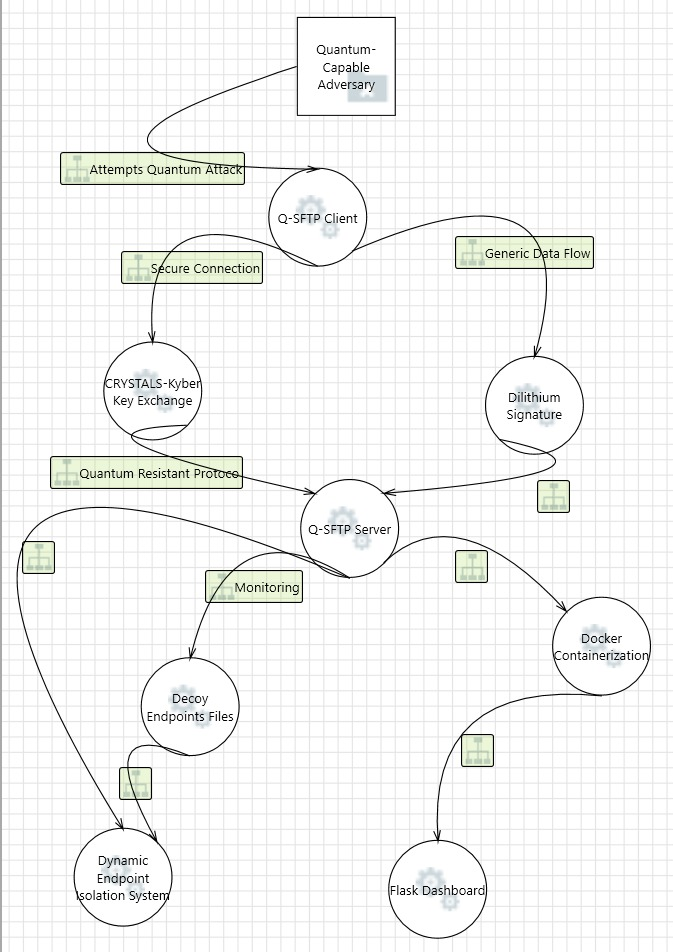
\includegraphics[width=0.88\textwidth]{Figures/threat_model.jpg}
    \caption{Threat Model of Quantum Secure FTP}
    \label{fig:threat}
\end{figure}

\section{Goals}

The main objectives of this project are:
\begin{enumerate}
    \item To design and implement a \textbf{four-phase PQC handshake protocol} using CRYSTALS-Kyber512 for key encapsulation and CRYSTALS-Dilithium2 for digital signatures, achieving mutual authentication and ephemeral session key derivation.
    
    \item To implement \textbf{BLAKE2b-256 file integrity verification} with dual-side hash comparison, a persistent hash registry, and periodic background integrity monitoring.
    
    \item To develop a \textbf{chunked resumable transfer protocol} with persistent state tracking, enabling reliable file transfer over unreliable network conditions.
    
    \item To enforce \textbf{role-based access control (RBAC)} with three tiers (Administrator, Standard, Guest) and per-user directory isolation.
    
    \item To provide \textbf{automatic metadata stripping} for privacy preservation and \textbf{malicious file protection} via extension blacklisting and magic number validation.
    
    \item To deploy the system as a \textbf{modern web application} with a browser-based GUI that abstracts all cryptographic complexity behind an intuitive interface.
\end{enumerate}


\section{Research Methodology}

The research is guided by the following questions:
\begin{enumerate}
    \item What are the vulnerabilities of contemporary SFTP protocols against quantum computing threats, and how does the ``Harvest Now, Decrypt Later'' model exacerbate these risks?
    
    \item How can NIST-standardized post-quantum cryptographic algorithms (CRYSTALS-Kyber and CRYSTALS-Dilithium) be integrated into a practical, deployable file transfer protocol?
    
    \item What additional security layers (file integrity, access control, metadata stripping, malicious file protection) are necessary for a production-grade post-quantum file transfer system?
    
    \item How does the performance of a PQC-based file transfer protocol compare to classical SFTP in terms of handshake latency, transfer throughput, and cryptographic overhead?
\end{enumerate}

\section{Structure of the Project}

The rest of the project is presented in the following chapters:

\begin{itemize}
    \item Chapter~\ref{chap.2} presents the preliminary background and related work: basics of secure file transfer, quantum-safe cryptography, and the Q-TLS handshake model.
    
    \item Chapter~\ref{chap.3} presents the results of the literature survey, comparing existing approaches, describing their limitations, and identifying the research gaps that motivated this project.
    
    \item Chapter~\ref{chap.4} presents the proposed system in detail: four-tier architecture, PQC handshake protocol (with formal mathematical notation), BLAKE2b integrity system, resumable chunked transfer protocol, file validation, metadata stripping, RBAC, activity logging, web GUI, admin panel, and deployment options.
    
    \item Chapter~\ref{chap.5} describes the key contributions, including a defense-in-depth analysis, novel findings during development, and a feature comparison with existing solutions.
    
    \item Chapter~\ref{chap.6} presents the experimental results: handshake verification, security testing, transfer performance evaluation, and comprehensive security analysis.
    
    \item Chapter~\ref{chap.7} concludes the project by summarizing achievements and discussing limitations.
    
    \item Chapter~\ref{chap.8} outlines future work including hybrid key exchange, formal verification, and WebSocket transport.
\end{itemize}

\chapter{Background}
\lhead{Chapter 2. \emph{Background}}
\label{chap.2}

This chapter provides the motivation for the construction of the Quantum Secure File Transfer Protocol (Q-SFTP). It reviews the history of secure file transfer methods, the cryptographic issues associated with these methods due to the advent of quantum computing, and the post-quantum techniques and handshake model upon which our system is built. 

\section{Secure File Transfer Protocols}

The protocol SFTP is a standard network protocol, used to securely transfer files over an encrypted session. It is implemented on top of the Secure Shell (SSH) protocol to provide confidentiality, integrity and authentication of data during transfer. However, security of the SFTP protocol relies on classical cryptographic algorithms such as RSA and Elliptic Curve Cryptography (ECC). Even though the above mentioned algorithms provide good protection against current computing threats, they remain susceptible to attacks from future quantum computers that will be able to break the underlying mathematical assumptions of these algorithms. This threat puts the long-term confidentiality of data transferred using classical encryption at risk. 

\section{Quantum Computing and Cryptographic Threats}

Quantum computing applies the principles of quantum mechanics, including superposition and entanglement, to perform complex computations in parallel.  Algorithms like Shor’s and Grover’s leverage these properties to efficiently solve mathematical problems that are currently intractable for classical computers.  Since the security of cryptographic systems such as RSA and ECC is based on these problems, the emergence of large-scale quantum computers will render such systems insecure.  This threat highlights the necessity of developing quantum-resistant cryptographic solutions that can protect data and communication in the post-quantum era. 

\section{Post-Quantum Cryptography}

Post-Quantum Cryptography (PQC) is a set of encryption and authentication algorithms that is assumed to be secure under the presence of classical and quantum adversaries. NIST has standardized a number of PQC schemes, such as the lattice-based key encapsulation scheme CRYSTALS-Kyber and the digital signature scheme CRYSTALS-Dilithium. Both schemes provide cryptographic primitives with strong security guarantees as well as good efficiency for implementation, which makes them ideal candidates to be incorporated into practical systems. In this project, we use these two schemes as the basis of the Quantum Secure File Transfer Protocol (Q-SFTP).

\section{File Transfer Protocol (FTP)}

The File Transfer Protocol (FTP) was one of the first standards developed for transferring files between clients and servers on a network. Although it provided a reliable way to exchange files between a client and server, it was sorely lacking in the area of encryption -- both the login credentials as well as the files were vulnerable to being intercepted.
Eventually, speaking of FTPS and SFTP, more security is added by adding encryption with SSL/TLS and SSH, but these use classical cryptographic systems, which are vulnerable to quantum attacks that break the mathematical assumptions.


\section{Quantum-TLS (Q-TLS) Handshake}

Q-SFTP provides an extra layer of security over top of Q-SFTP’s Quantum Transport Layer Security (Q-TLS) handshake, which is somewhat analogous in purpose to the TLS protocol. While TLS might use RSA or Elliptic Curve Diffie-Hellman (ECDHE) to provide a session key exchange that is quantum resistant, Q-SFTP uses CRYSTALS-Kyber. Thereafter an analogous process provides the authentication portion of the handshake via CRYSTALS-Dilithium digital signatures.

\chapter{Literature Survey}
\lhead{Chapter 3. \emph{Literature Survey}}
\label{chap.3}

 The literature survey discusses the existing research works and technologies which motivated the proposed Quantum Secure File Transfer Protocol (Q-SFTP). The Literature Survey section discusses the traditional file transfer protocols, post-quantum cryptographic standards, secure communication framework and the research gap motivated for this work.

\section{Existing Secure File Transfer Mechanisms}

The traditional methods of transferring files such as FTP, FTPS and SFTP have been used for exchanging data with other entities over the network for many years. Since FTP does not provide any encryption, it can be seen that the data transferred using this method is vulnerable to an attacker. Later, FTPS has been achieved by using TLS, and SFTP has been used SSH for the encrypted sessions. In \cite{krawczyk2020tls13} and \cite{bos2023pqftp} it has been shown that these protocols are sufficiently secure against classical attacks, but since they depend on RSA and ECC, they are useless in the post-quantum era. Therefore, the previous systems are useless in providing confidentiality and integrity of the data when the quantum computers become usable.

\section{Post-Quantum Cryptographic Developments}

New results in Post-Quantum Cryptography (PQC).
Post-Quantum Cryptography refers to cryptographic algorithms that are secure against an adversary possessing a quantum computer. NIST has started a standardization process to detect robust and efficient PQC algorithms. So far CRYSTALS-Kyber and CRYSTALS-Dilithium have been identified as efficient key encapsulation and key-secure digital signatures respectively \cite{avanzi2021kyber, dam2023survey}. Both are lattice-based key-establishment algorithms with strong security assumptions and good efficiency criteria, that can be implemented in current communication protocols.

\section{Quantum-Resilient Communication Protocols}

Several works have investigated how to extend current communication systems with quantum-safe cryptography. These approaches include using hybrid TLS models that apply classical and post-quantum algorithms to gain backward compatibility while enhancing resistance against quantum attacks. However, these approaches are still mostly in the design or experimental phases, and their real implementations are scarce. Furthermore, few works have evaluated their performance in practical network environments. These results motivate the design and implementation of a deployable post-quantum secure file transfer protocol.

\section{Research Gap and Motivation}

Although there has been considerable research on post-quantum cryptography, its adoption in secure file transfer systems is scarce. Most of the existing works either lean towards the design of cryptographic algorithms or consider general-purpose communication protocols, not taking into account file transfer efficiency, session handling, nor usability. In this work, we fill this gap by formulating and implementing a Quantum Secure File Transfer Protocol (Q-SFTP) that integrates practical quantum-resistant cryptographic primitives into an efficient and secure client-server file transfer system with theoretical guarantees in both directions \cite{sola2025quantumftp, baseri2024navigating}.

\chapter{Proposed Methods}
\lhead{Chapter 4. \emph{Proposed Methods}}
\label{chap.4}

This chapter presents the design, architecture, and implementation methodology of the Quantum Secure File Transfer Protocol (Q-SFTP). The system is built as a four-tier modular architecture integrating NIST-standardized post-quantum cryptographic (PQC) primitives with production-grade features including file integrity verification, resumable chunked transfers, role-based access control, metadata stripping, and a modern web interface.

\section{System Architecture}

Q-SFTP employs a four-tier, modularized architecture to protect confidentiality, integrity, and authentication of data in a post-quantum world. The four tiers are:

\begin{enumerate}
    \item \textbf{Client Layer (Web Browser):} A single-page web application using HTML5, CSS3, and vanilla JavaScript. Client-side BLAKE2b hashing is performed using the \texttt{blakejs} library. Transfer state persistence uses the browser's \texttt{localStorage} API, enabling resume across page reloads and session restarts.
    
    \item \textbf{Application Layer (Flask Web Server):} The Flask 3.x web server on port 5000 serves as the middleware between the browser and the PQC transport layer. It manages user authentication, transfer coordination, hash verification, privacy management, activity logging, and the admin panel.
    
    \item \textbf{Transport Layer (PQC Handshake Server):} The handshake server listens on TCP port 8888 and implements the four-phase Q-TLS handshake protocol using CRYSTALS-Kyber512 for key encapsulation and CRYSTALS-Dilithium2 for digital signatures. All file operations are routed through this encrypted channel.
    
    \item \textbf{Storage Layer (ServerStorage):} Server-side storage follows a directory-isolation model where each user has a private directory, plus a shared collaborative directory accessible to all authenticated users.
\end{enumerate}

Figure~\ref{fig:architecture} illustrates the overall structure of the Q-SFTP framework.

\begin{figure}[H]
    \centering
    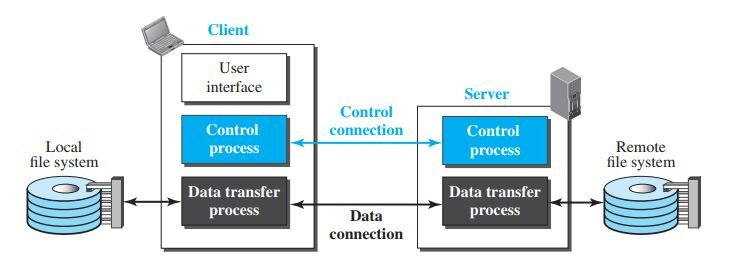
\includegraphics[width=0.85\textwidth]{Figures/FTP-architecture.png}
    \caption{Overall System Architecture of Q-SFTP}
    \label{fig:architecture}
\end{figure}

\section{Certificate Authority Design}

The Certificate Authority (CA) is a lightweight, self-contained module that issues and verifies post-quantum digital certificates using CRYSTALS-Dilithium. Unlike classical X.509 certificates that rely on RSA or ECDSA, the CA in Q-SFTP uses Dilithium2 for both signature generation and verification.

\begin{figure}[H]
    \centering
    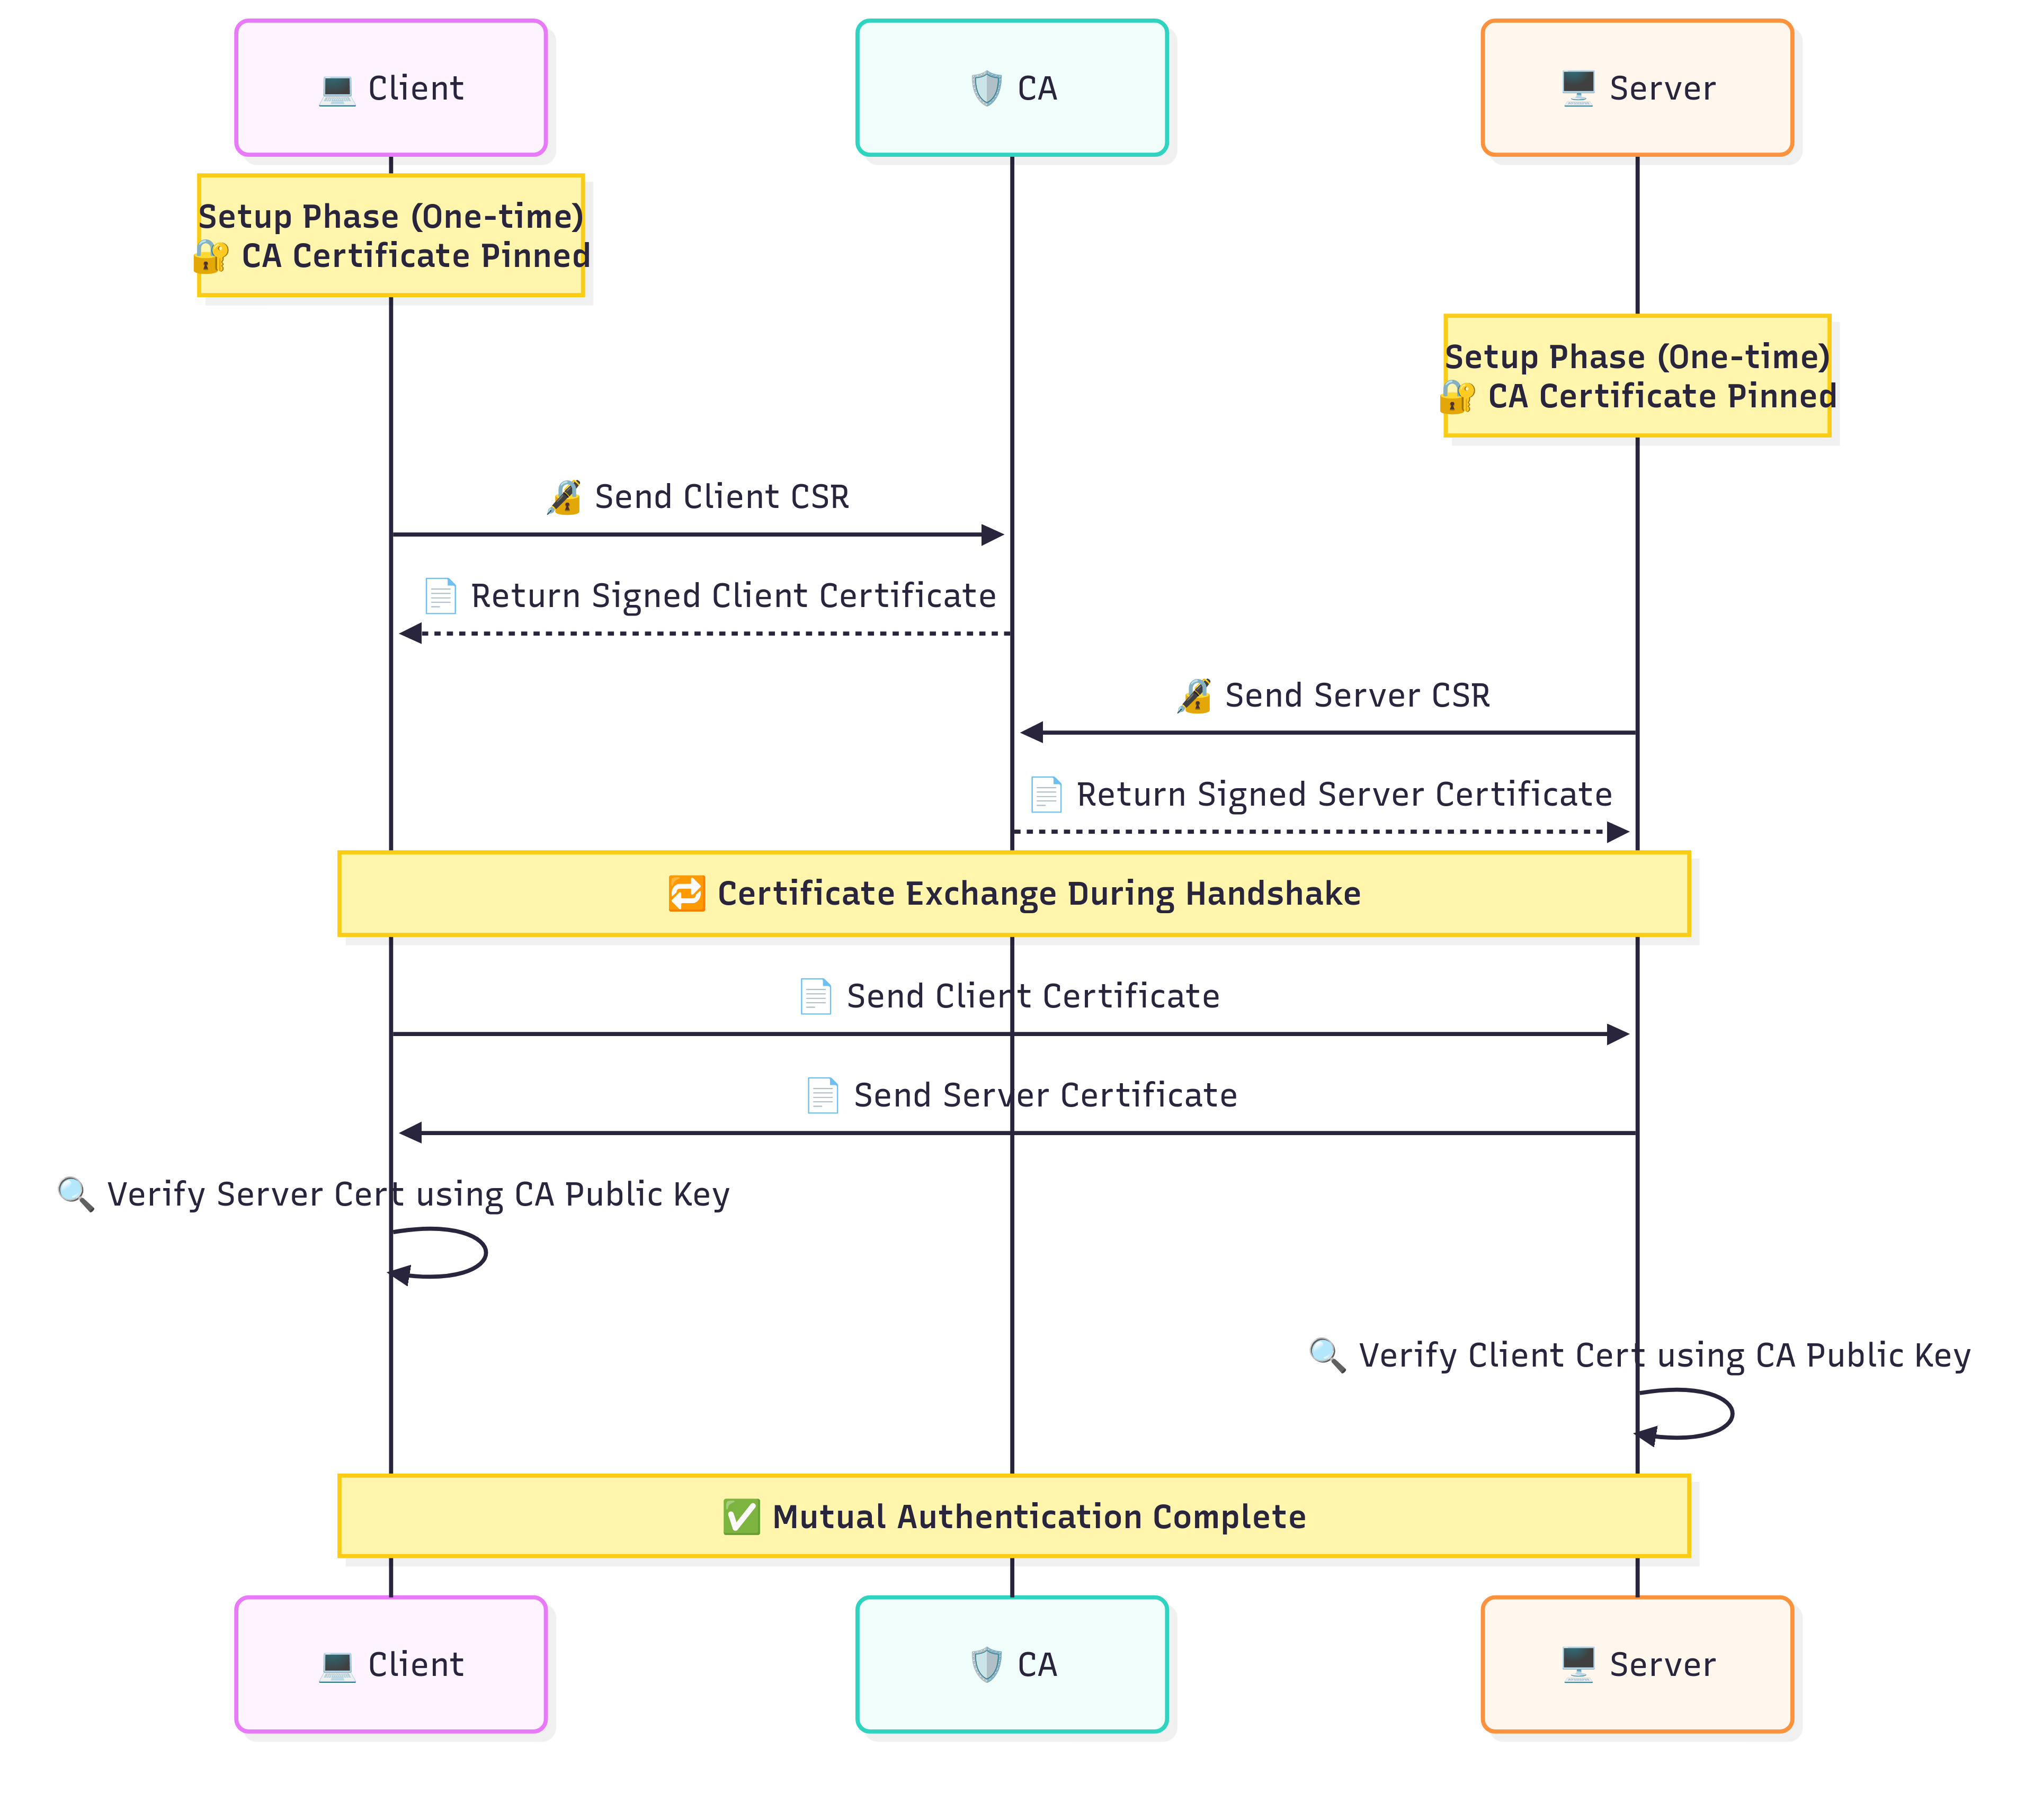
\includegraphics[width=0.8\textwidth]{Figures/CA.png}
    \caption{Architecture of the Quantum-Safe Certificate Authority}
    \label{fig:ca_architecture}
\end{figure}

\subsection{Certificate Format (Q-Cert)}

The custom certificate format retains common X.509 fields while adding support for post-quantum public keys and signatures:

\begin{itemize}
    \item \textbf{Subject:} Entity identifier (e.g., ``Server'', ``admin'', ``bob'')
    \item \textbf{Issuer:} CA identifier
    \item \textbf{Public\_Key:} Hex-encoded Dilithium2 public key (1,312 bytes)
    \item \textbf{Valid\_From / Valid\_Until:} ISO 8601 validity period
    \item \textbf{Signature:} Dilithium2 signature over all preceding fields
\end{itemize}

\begin{figure}[H]
    \centering
    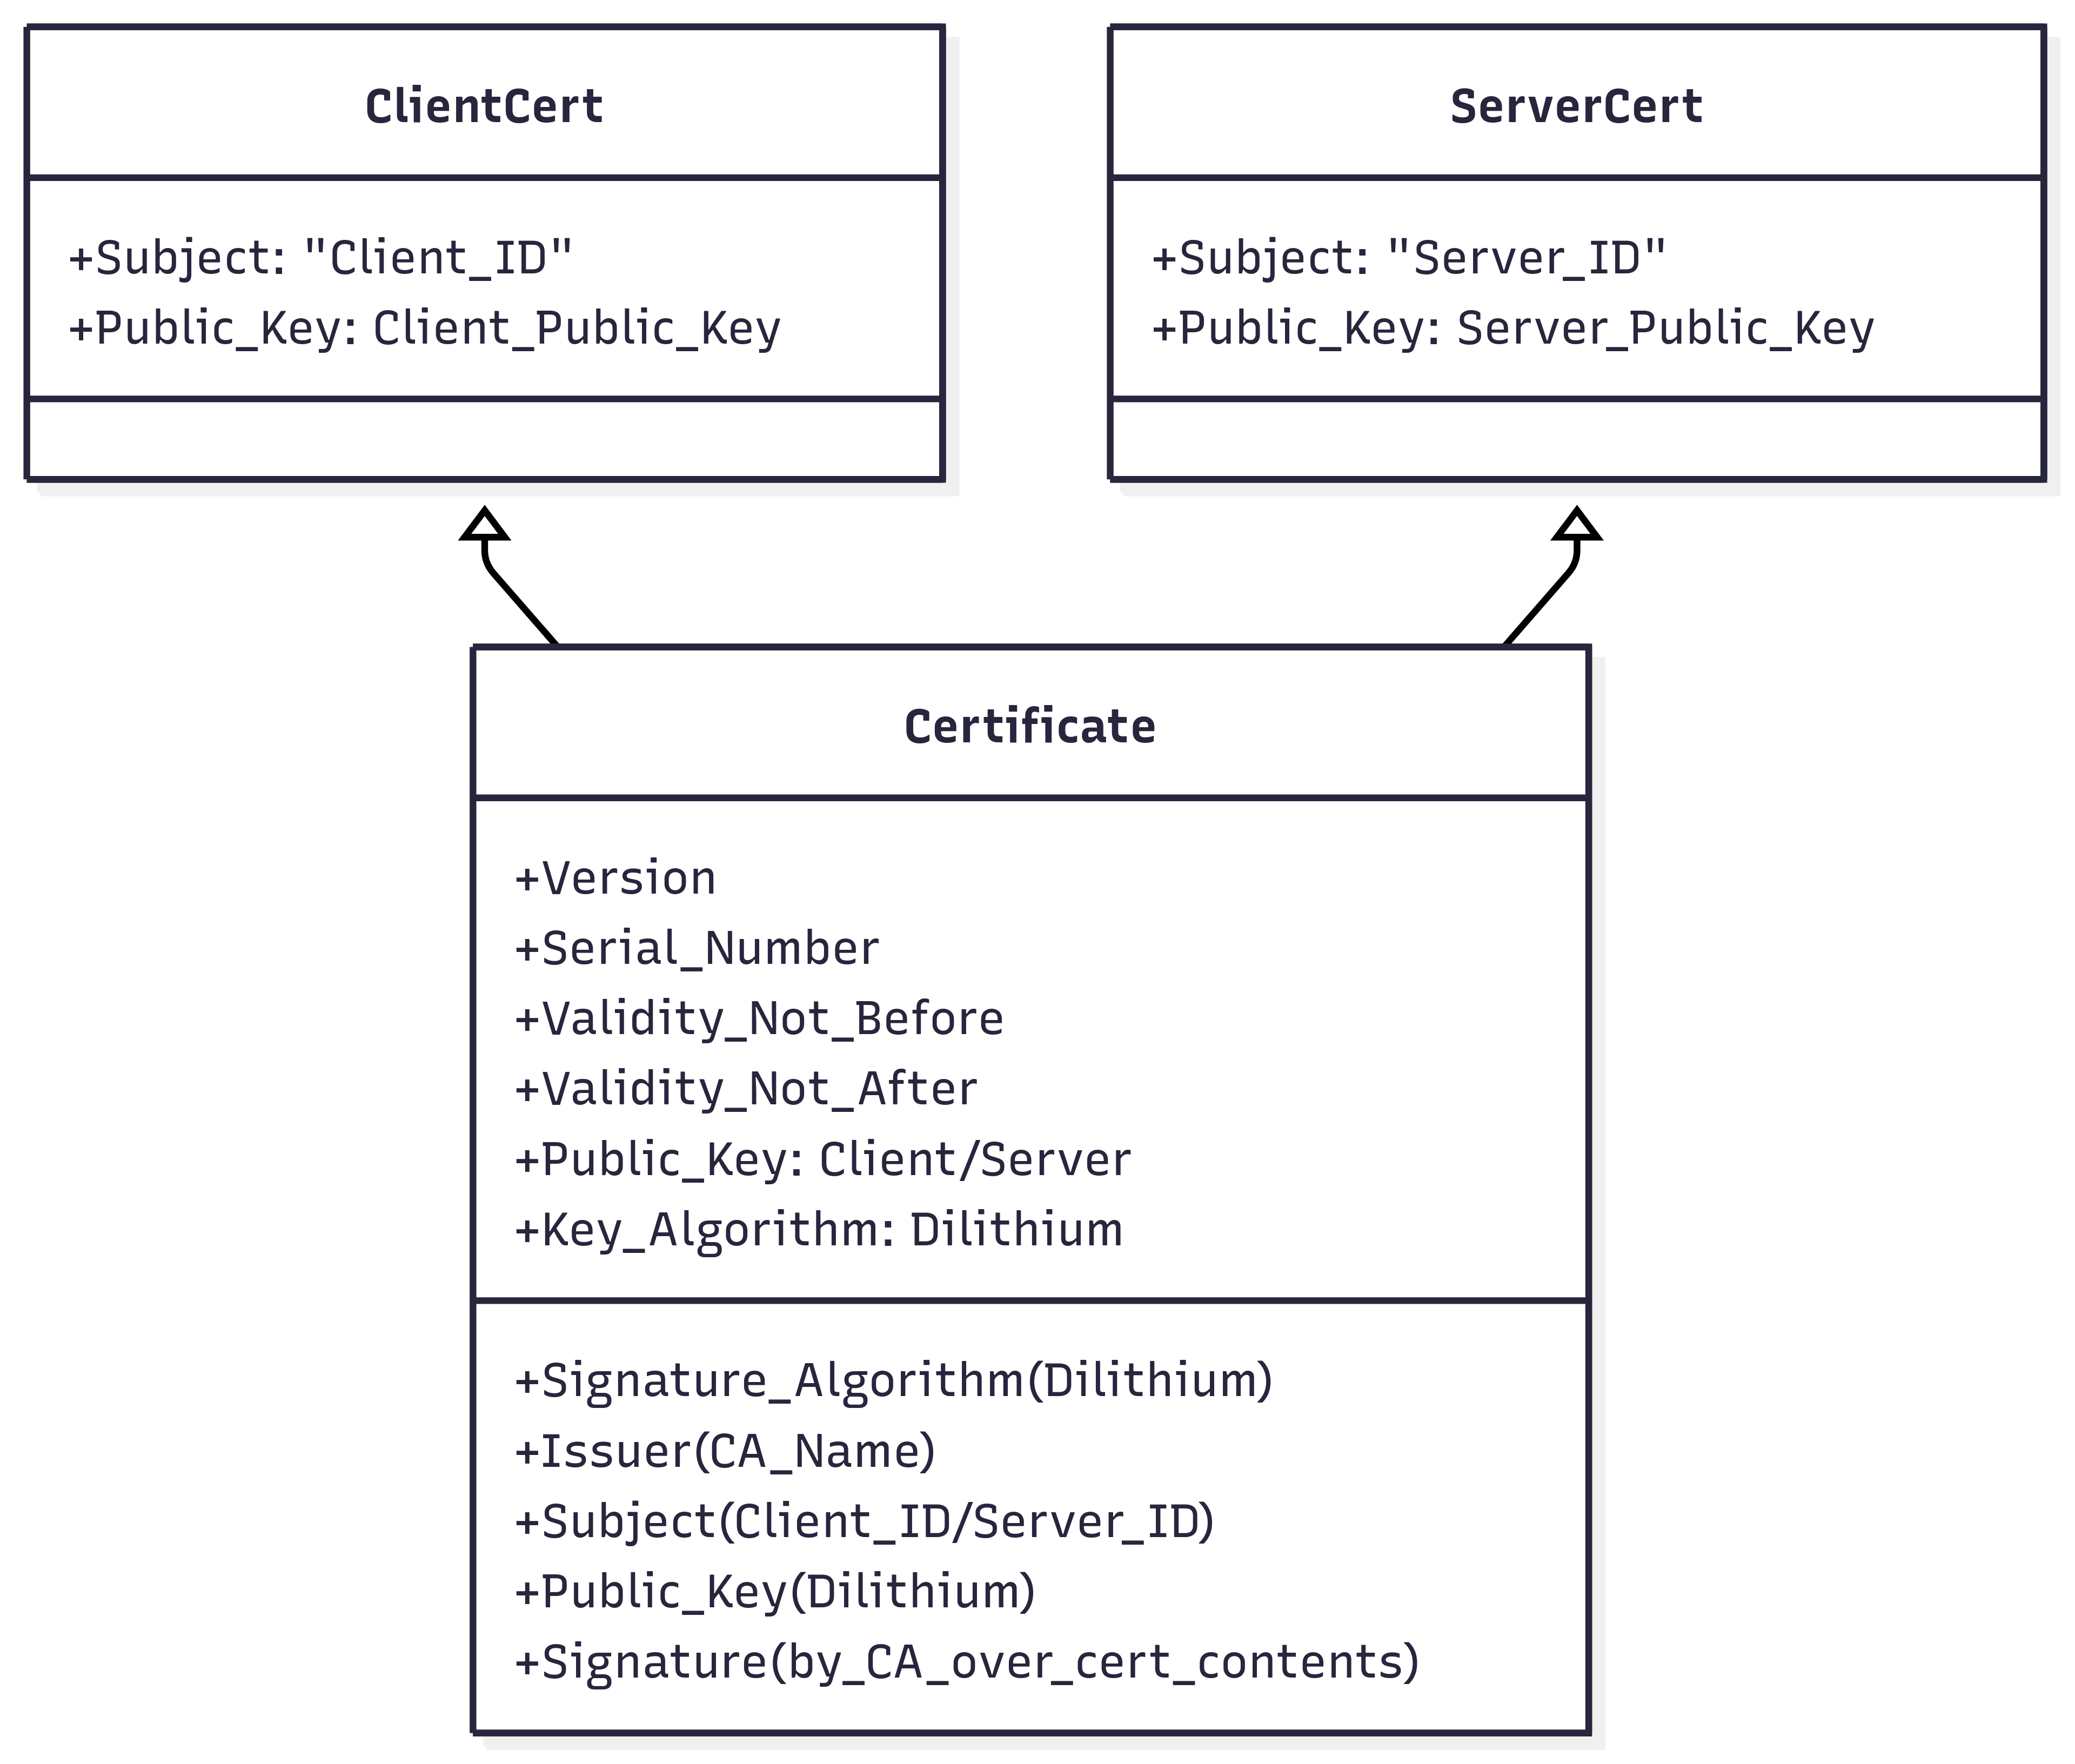
\includegraphics[width=0.75\textwidth]{Figures/Certificate.png}
    \caption{Structure of the Post-Quantum Digital Certificate (Q-Cert)}
    \label{fig:certificate_format}
\end{figure}

\section{Q-TLS Handshake Protocol}

The Q-TLS handshake replaces classical RSA/ECDHE-based key exchange with CRYSTALS-Kyber512 and uses Dilithium2 for mutual authentication. The protocol operates in four phases:

\subsection{Phase 1: Hello Exchange}

\begin{enumerate}
    \item The client generates a random nonce $N_C$ and a UTC timestamp $T_C$, then sends a \textit{ClientHello} message containing its digital certificate, nonce, and timestamp.
    \item The server verifies the client certificate against the CA's public key, checks that $|T_S - T_C| < 30$ seconds (replay protection), and generates a Kyber512 key pair $(pk_{Kyber}, sk_{Kyber})$.
    \item The server creates a Dilithium2 signature over the concatenation of $N_C$, its own nonce $N_S$, and $pk_{Kyber}$:
    \[
    \sigma_S = \text{Dilithium2.Sign}(sk_S^{Dil}, N_C \| N_S \| pk_{Kyber})
    \]
    \item The server responds with a \textit{ServerHello} containing its certificate, Kyber public key, nonce, and signature.
\end{enumerate}

\subsection{Phase 2: Key Encapsulation (Kyber512)}

\begin{enumerate}
    \item The client verifies $\sigma_S$, then encapsulates a shared secret using the server's Kyber public key:
    \[
    (ct, ss) = \text{Kyber512.Encaps}(pk_{Kyber})
    \]
    \item The client sends $ct$ (ciphertext, 768 bytes) to the server.
    \item The server decapsulates to recover the shared secret:
    \[
    ss = \text{Kyber512.Decaps}(sk_{Kyber}, ct)
    \]
\end{enumerate}

\subsection{Phase 3: Mutual Authentication and Key Derivation}

\begin{enumerate}
    \item The client computes a transcript hash over all exchanged messages:
    \[
    h_{transcript} = \text{SHA-256}(\text{ClientHello} \| \text{ServerHello} \| \text{ClientKeyShare})
    \]
    \item The client signs the transcript hash: $\sigma_C = \text{Dilithium2.Sign}(sk_C^{Dil}, h_{transcript})$
    \item The server verifies $\sigma_C$, confirming mutual authentication.
    \item Both parties derive the session key:
    \[
    K_{session} = \text{HKDF-SHA256}(ss, \text{salt} = \text{SHA-256}(N_C \| N_S), \text{info} = \text{``Q-SFTP-SESSION-KEY''})
    \]
\end{enumerate}

\subsection{Phase 4: Secure Data Transfer}

All subsequent communication is encrypted with AES-256-GCM using $K_{session}$, where each message uses a unique 96-bit nonce. The GCM authentication tag provides both confidentiality and integrity.

\begin{figure}[p]
    \centering
    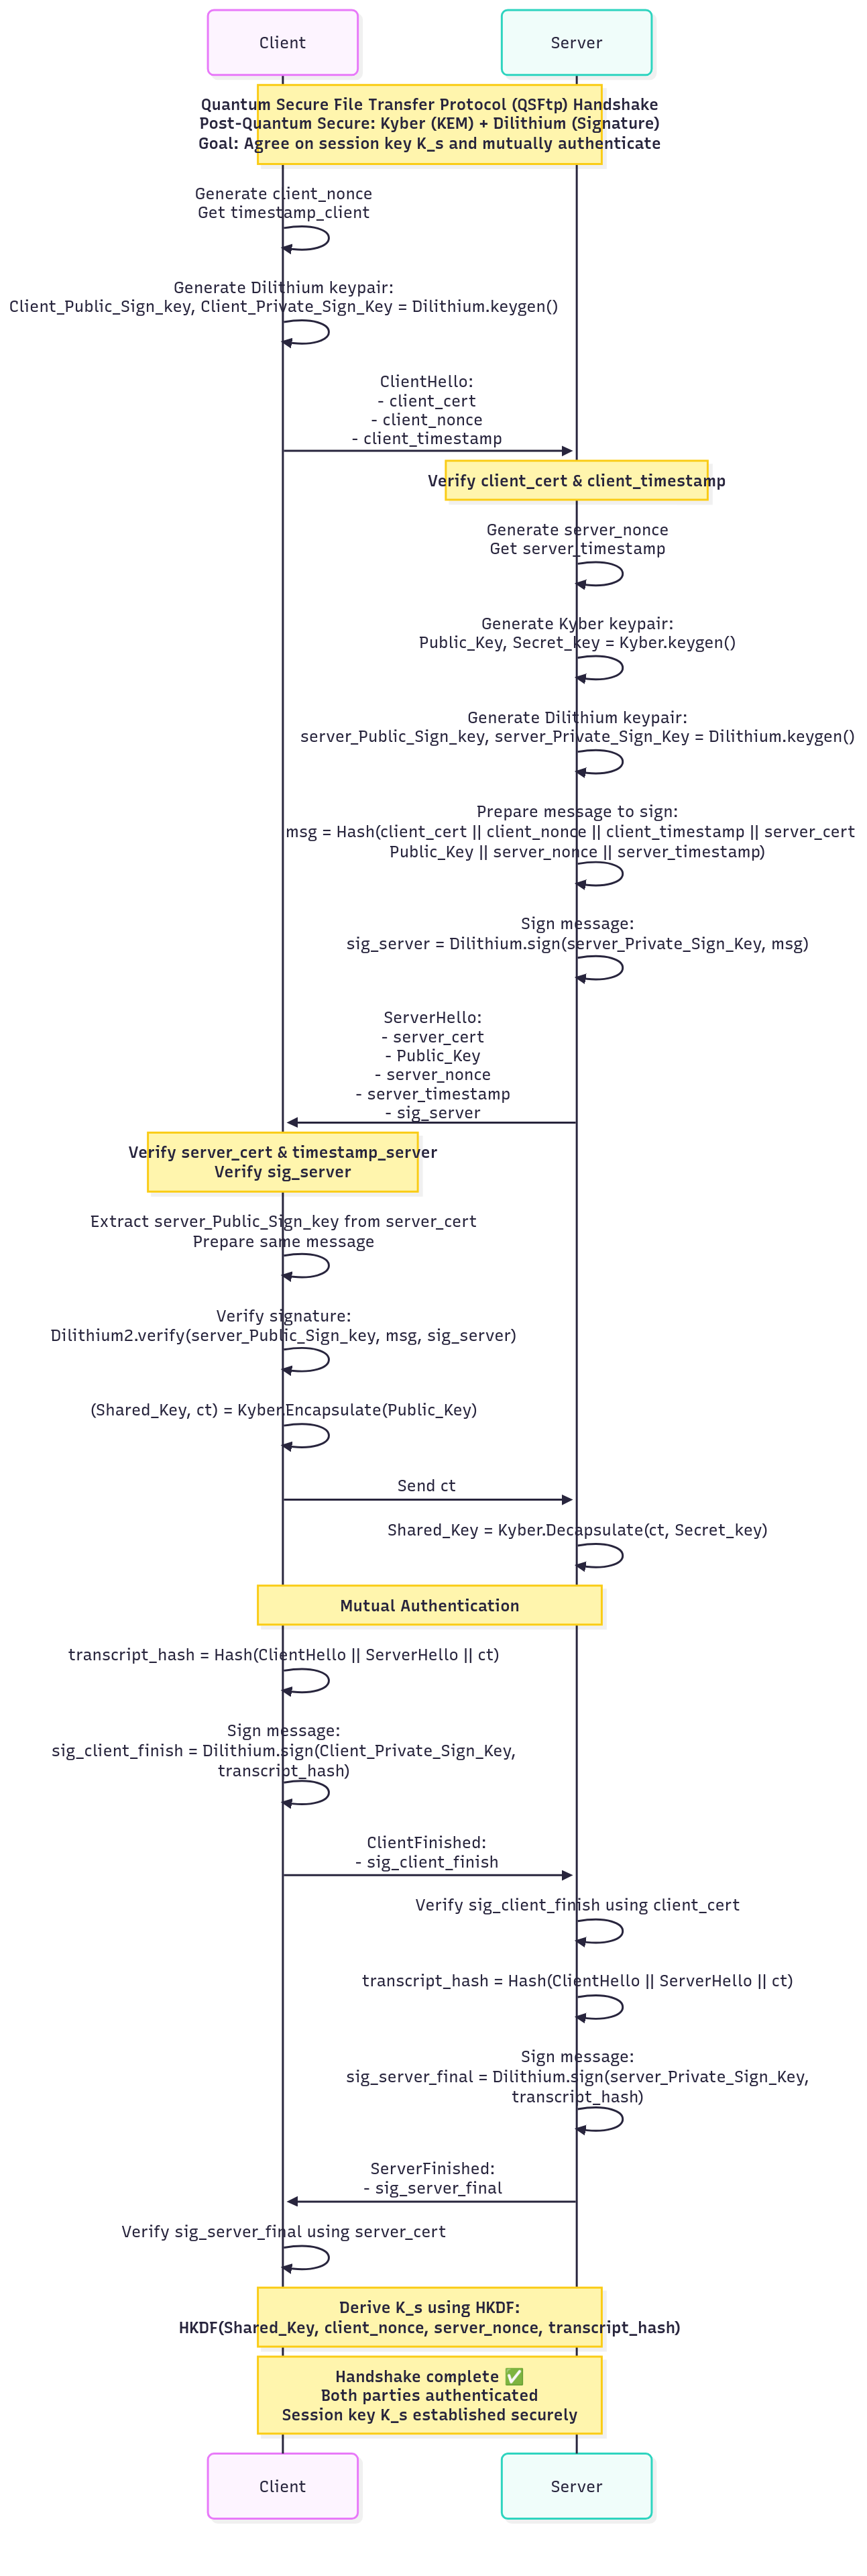
\includegraphics[height=\textheight]{Figures/Handshake.png}
    \caption{Proposed Quantum-TLS (Q-TLS) Handshake Sequence}
    \label{fig:handshake}
\end{figure}

\subsection{Handshake Algorithm}

Algorithm~\ref{algo:handshake} summarizes the Q-TLS handshake procedure.

\begin{algorithm}[H]
\caption{Q-TLS Handshake Protocol}
\label{algo:handshake}
\begin{algorithmic}[1]
\State Client generates $(N_C, T_C)$
\State Client $\rightarrow$ Server: \textit{ClientHello}(Cert$_C$, $N_C$, $T_C$)
\State Server verifies Cert$_C$ via CA public key
\State Server generates $(pk_{Kyber}, sk_{Kyber})$ and $N_S$
\State Server signs: $\sigma_S \gets$ Dilithium2.Sign($sk_S$, $N_C \| N_S \| pk_{Kyber}$)
\State Server $\rightarrow$ Client: \textit{ServerHello}(Cert$_S$, $pk_{Kyber}$, $N_S$, $\sigma_S$)
\State Client verifies Cert$_S$ and $\sigma_S$
\State Client: $(ct, ss) \gets$ Kyber512.Encaps($pk_{Kyber}$)
\State Client $\rightarrow$ Server: \textit{ClientKeyShare}($ct$)
\State Server: $ss \gets$ Kyber512.Decaps($sk_{Kyber}$, $ct$)
\State Client computes $h_{tr} \gets$ SHA-256(transcript)
\State Client signs: $\sigma_C \gets$ Dilithium2.Sign($sk_C$, $h_{tr}$)
\State Client $\rightarrow$ Server: \textit{ClientFinished}($\sigma_C$, $h_{tr}$)
\State Server verifies $\sigma_C$ \Comment{Mutual authentication complete}
\State Both derive: $K \gets$ HKDF-SHA256($ss$, SHA-256($N_C \| N_S$))
\State \textbf{Begin} AES-256-GCM encrypted communication
\end{algorithmic}
\end{algorithm}

\section{File Integrity Verification (BLAKE2b)}

Q-SFTP implements a comprehensive file integrity verification system using BLAKE2b-256 hashing, applied at multiple stages of the file lifecycle.

\subsection{Hash Computation}

BLAKE2b-256 was selected over SHA-256 for file hashing due to its superior performance (approximately 3$\times$ faster on modern processors) while maintaining equivalent security margins. The hash is computed as:
\[
H_{file} = \text{BLAKE2b}(\text{file\_data}, \text{digest\_size} = 32)
\]

On the client side, the \texttt{blakejs} JavaScript library provides in-browser BLAKE2b computation.

\subsection{Dual-Side Verification}

\begin{enumerate}
    \item \textbf{Upload verification}: The client computes $H_{client}$ before upload. The server independently computes $H_{server}$ after reception. A mismatch indicates transmission corruption.
    \item \textbf{Download verification}: The server retrieves the stored hash $H_{stored}$ and computes the current hash $H_{current}$. If $H_{stored} = H_{current}$, the file status is \texttt{VERIFIED}; otherwise, \texttt{TAMPERED}.
\end{enumerate}

\subsection{Persistent Hash Registry}

All file hashes are stored in a JSON-based registry (\texttt{hash\_registry.json}) containing: file ID (UUID), file path, BLAKE2b hash (hex), algorithm identifier, registering username, timestamp, and file size.

\subsection{Background Integrity Checker}

The \texttt{IntegrityChecker} module runs periodic background scans (configurable interval, default 3600 seconds) that re-verify all registered files against stored hashes. Any unauthorized modifications are detected and flagged.

Algorithm~\ref{algo:integrity} describes the hash verification procedure.

\begin{algorithm}[H]
\caption{BLAKE2b File Integrity Verification}
\label{algo:integrity}
\begin{algorithmic}[1]
\Require File $F$, Hash Registry $R$
\State $H_{current} \gets \text{BLAKE2b-256}(F.\text{data})$
\If{$F.\text{path} \in R$}
    \State $H_{stored} \gets R[F.\text{path}].\text{hash}$
    \If{$H_{current} = H_{stored}$}
        \State \Return \texttt{VERIFIED}
    \Else
        \State \Return \texttt{TAMPERED}
    \EndIf
\Else
    \State Register $(F.\text{path}, H_{current})$ in $R$
    \State \Return \texttt{NEW}
\EndIf
\end{algorithmic}
\end{algorithm}

\section{Resumable Chunked Transfer Protocol}

Traditional file transfer protocols transmit files as monolithic blobs, making them vulnerable to connection interruptions. Q-SFTP introduces a chunked, resumable transfer protocol that operates within the PQC-encrypted channel.

\subsection{Protocol Design}

Files are divided into fixed-size chunks of $C = 256$ KB (262,144 bytes). Each chunk is independently encrypted with AES-256-GCM before transmission. The protocol uses five REST API endpoints:

\begin{itemize}
    \item \texttt{POST /api/upload/init} — Initialize an upload session; returns \texttt{transfer\_id} and optional \texttt{resume\_offset}.
    \item \texttt{POST /api/upload/chunk} — Send a single chunk with offset and optional \texttt{IsFinal} flag.
    \item \texttt{POST /api/upload/complete} — Finalize the upload, rename \texttt{.part} file, and register hash.
    \item \texttt{POST /api/download/init} — Initialize a download session; returns file size and hash.
    \item \texttt{POST /api/download/chunk} — Retrieve chunk at a given offset.
\end{itemize}

\subsection{Transfer State Persistence}

The \texttt{TransferManager} maintains a persistent log (\texttt{transfer\_log.json}) with the following state per transfer:

\begin{table}[H]
    \centering
    \caption{Transfer log entry fields}
    \label{tab:transfer}
    \begin{tabular}{|l|l|p{7cm}|}
        \hline
        \textbf{Field} & \textbf{Type} & \textbf{Description} \\
        \hline
        \texttt{transfer\_id} & UUID & Unique session identifier \\
        \hline
        \texttt{filename} & String & Original filename \\
        \hline
        \texttt{total\_size} & Integer & Total file size in bytes \\
        \hline
        \texttt{bytes\_transferred} & Integer & Confirmed bytes transferred \\
        \hline
        \texttt{chunk\_size} & Integer & Chunk size (default: 262,144 B) \\
        \hline
        \texttt{status} & Enum & \texttt{active} $|$ \texttt{complete} $|$ \texttt{failed} \\
        \hline
        \texttt{direction} & Enum & \texttt{upload} $|$ \texttt{download} \\
        \hline
    \end{tabular}
\end{table}

\subsection{Resume Semantics}

When a transfer is initiated, the \texttt{TransferManager} checks for an existing active session matching the tuple (filename, username, remote\_path, direction). If found, the server returns the saved \texttt{bytes\_transferred} as \texttt{resume\_offset}. On the client side, \texttt{localStorage} stores a mirror of the transfer state.

\subsection{Upload Process}

Algorithm~\ref{algo:upload} describes the chunked upload procedure.

\begin{algorithm}[H]
\caption{Chunked Resumable Upload}
\label{algo:upload}
\begin{algorithmic}[1]
\Require File $F$, chunk size $C = 256$ KB
\State $H_{client} \gets \text{BLAKE2b-256}(F)$
\State $(transfer\_id, offset) \gets \text{POST /api/upload/init}(F.\text{name}, |F|, H_{client})$
\While{$offset < |F|$}
    \State $chunk \gets F[offset : offset + C]$
    \State $is\_final \gets (offset + C \geq |F|)$
    \State Send chunk via PQC-encrypted \texttt{ChunkUpload} message
    \State $offset \gets offset + |chunk|$
    \State Save $offset$ to \texttt{localStorage}
\EndWhile
\State POST /api/upload/complete($transfer\_id$)
\State Server renames \texttt{.part} $\rightarrow$ final filename
\State Server registers $H_{server}$ in hash registry
\end{algorithmic}
\end{algorithm}

\section{Malicious File Protection}

The \texttt{FileValidator} module implements defense-in-depth against malicious uploads:

\begin{enumerate}
    \item \textbf{Extension Blacklisting:} 17 dangerous file extensions are blocked: \texttt{.exe}, \texttt{.dll}, \texttt{.scr}, \texttt{.com}, \texttt{.msi}, \texttt{.cmd}, \texttt{.vbs}, \texttt{.vbe}, \texttt{.wsf}, \texttt{.wsh}, \texttt{.pif}, \texttt{.cpl}, \texttt{.inf}, \texttt{.reg}, \texttt{.sys}, \texttt{.drv}, \texttt{.ocx}.
    
    \item \textbf{Magic Number Validation:} For 20+ known binary formats (JPEG, PNG, GIF, PDF, ZIP, DOCX, XLSX, MP3, MP4, etc.), the file's initial bytes are verified against expected magic number signatures, preventing extension spoofing attacks.
    
    \item \textbf{First-Chunk Validation:} For chunked uploads, validation occurs on the first chunk where file headers reside.
\end{enumerate}

\section{Metadata Stripping and Privacy Preservation}

The \texttt{PrivacyManager} module automatically removes potentially identifying metadata before files are stored on the server:

\begin{itemize}
    \item \textbf{Images (JPEG/PNG):} EXIF data (GPS coordinates, camera model, timestamps) is stripped using Pillow while preserving image quality.
    \item \textbf{PDF Documents:} Author, title, subject, creator, producer, and modification dates are removed using PyPDF2.
    \item \textbf{Word Documents (.docx):} Author, last modified by, company, and other core properties are sanitized using python-docx.
    \item \textbf{IP Anonymization:} Client IP addresses in activity logs are hashed with a daily rotating salt using SHA-256, preventing long-term tracking.
\end{itemize}

\section{Role-Based Access Control (RBAC)}

Q-SFTP implements a three-tier RBAC model enforced at the handshake server level.

\subsection{Role Definitions}

\begin{table}[H]
    \centering
    \caption{RBAC permission matrix}
    \label{tab:rbac}
    \begin{tabular}{|l|c|c|c|}
        \hline
        \textbf{Operation} & \textbf{Administrator} & \textbf{Standard} & \textbf{Guest} \\
        \hline
        List Files (READ) & \checkmark & \checkmark & \checkmark \\
        \hline
        Download (READ) & \checkmark & \checkmark & \checkmark \\
        \hline
        Upload (WRITE) & \checkmark & \checkmark & $\times$ \\
        \hline
        Create Directory (WRITE) & \checkmark & \checkmark & $\times$ \\
        \hline
        Delete (DELETE) & \checkmark & \checkmark & $\times$ \\
        \hline
        Admin Panel (ALL) & \checkmark & $\times$ & $\times$ \\
        \hline
    \end{tabular}
\end{table}

\subsection{Directory Isolation}

Each user's files are stored in an isolated directory (\texttt{ServerStorage/\{username\}/}), preventing unauthorized cross-user access. A shared directory (\texttt{ServerStorage/shared/}) provides collaborative storage accessible to all authenticated users with appropriate permissions.

\subsection{Authentication} 

User credentials are stored in a SQLite database (\texttt{users.db}) with passwords hashed using PBKDF2-HMAC-SHA256 with 100,000 iterations and a random salt.

\section{Activity Logging and Audit Trail}

The \texttt{ActivityLogger} module maintains a comprehensive, thread-safe audit log stored in an SQLite database (\texttt{activity\_logs.db}):

\begin{itemize}
    \item \textbf{Logged events:} Login success/failure, file uploads, downloads, deletions, directory creation, admin actions.
    \item \textbf{Recorded metadata:} Anonymized IP, username, action type, filename, timestamp, file size.
    \item \textbf{Privacy:} IP addresses are anonymized via SHA-256 with a daily rotating salt.
    \item \textbf{Tamper detection:} Log chain integrity is verified using hash chaining of sequential entries.
    \item \textbf{Query support:} Logs can be filtered by user, date range, action type, and IP prefix.
\end{itemize}

\section{Web Application and Admin Panel}

\subsection{Web GUI}

The web application provides a modern, browser-based interface for file management:

\begin{itemize}
    \item \textbf{File browser:} Remote directory listing with breadcrumb navigation.
    \item \textbf{Multi-file upload:} Drag-and-drop or button-based multi-file upload with progress bars.
    \item \textbf{Bulk operations:} Select-all and multi-file download/delete.
    \item \textbf{Transfer queue:} Visual progress indicators for all active transfers.
    \item \textbf{Security status:} Real-time display of connection security (PQC algorithm in use, session key status, hash verification results).
    \item \textbf{Theme switching:} Dark/light mode toggle with CSS custom properties.
\end{itemize}

\subsection{Admin Panel}

Available only to users with the Administrator role:

\begin{itemize}
    \item \textbf{User management:} Create, delete, and role-assign users.
    \item \textbf{Activity logs:} Searchable, filterable audit trail viewer.
    \item \textbf{Integrity dashboard:} View hash verification status for all files.
    \item \textbf{System status:} Connection state, handshake details, and server health.
\end{itemize}

\section{Deployment}

Q-SFTP supports three deployment modes:

\begin{enumerate}
    \item \textbf{Local:} A batch script (\texttt{start\_q\_sftp.bat}) launches both the handshake server and Flask web application.
    \item \textbf{Docker:} A single container exposing ports 5000 (web) and 8888 (handshake), built from a lightweight Python 3.12 base image.
    \item \textbf{Docker Compose:} Multi-container orchestration with volume mounts for persistent storage.
\end{enumerate}

\section{Architectural Diagrams}

This section presents the key architectural and workflow diagrams that illustrate the core subsystems of Q-SFTP.

\subsection{System Architecture Overview}

Figure~\ref{fig:arch_diagram} provides a high-level view of the four-tier Q-SFTP architecture, showing the interaction between the client browser, Flask application server, PQC handshake server, and the storage layer.

\begin{figure}[H]
    \centering
    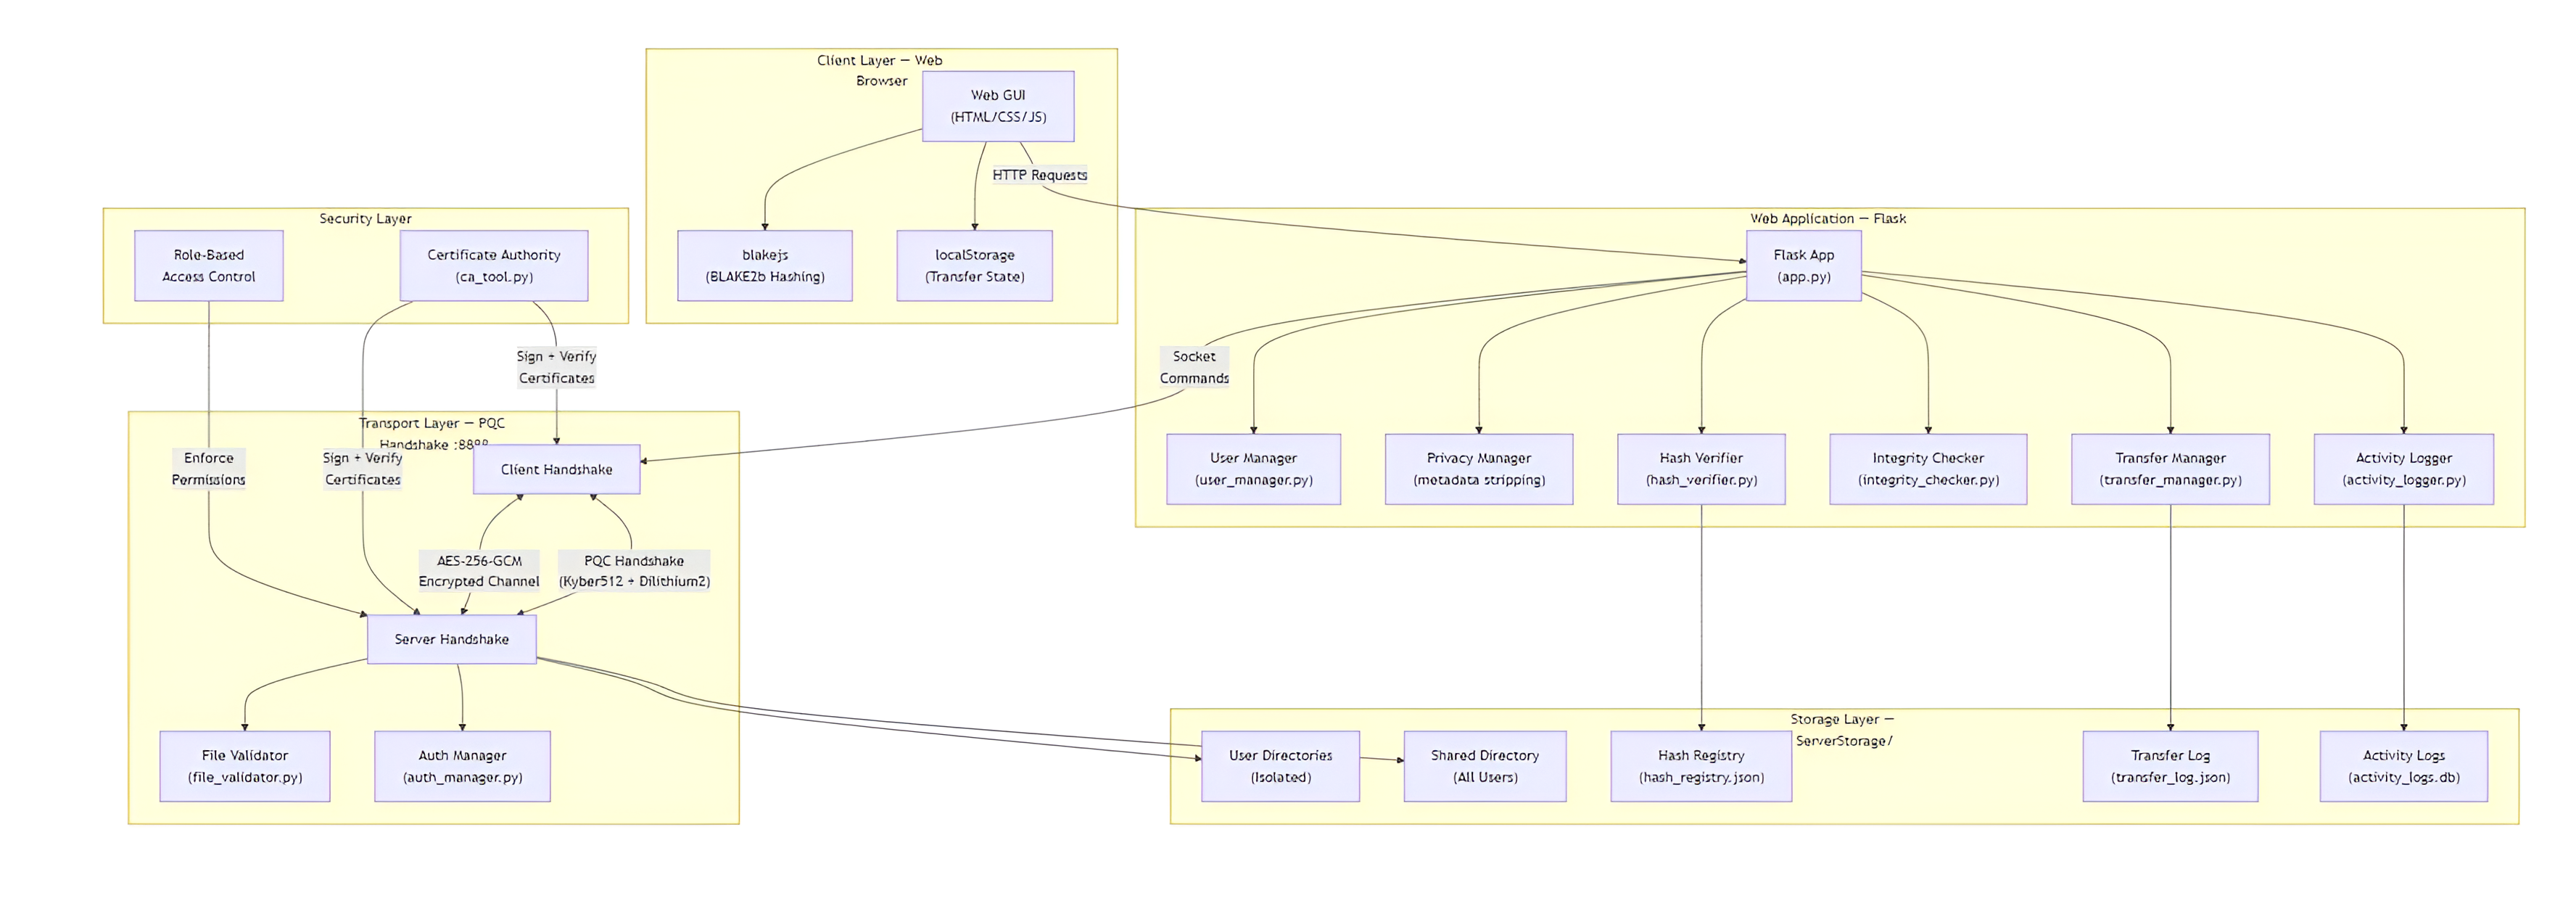
\includegraphics[width=\textwidth]{Figures/System_Architecture.png}
    \caption{Q-SFTP System Architecture — Four-Tier Modular Design}
    \label{fig:arch_diagram}
\end{figure}

\subsection{PQC Handshake Protocol Flow}

Figure~\ref{fig:pqc_diagram} illustrates the four-phase post-quantum handshake protocol: Hello Exchange, Kyber512 Key Encapsulation, Mutual Authentication via Dilithium2 transcript signing, and Secure Channel Establishment with HKDF-derived session keys.

\begin{figure}[H]
    \centering
    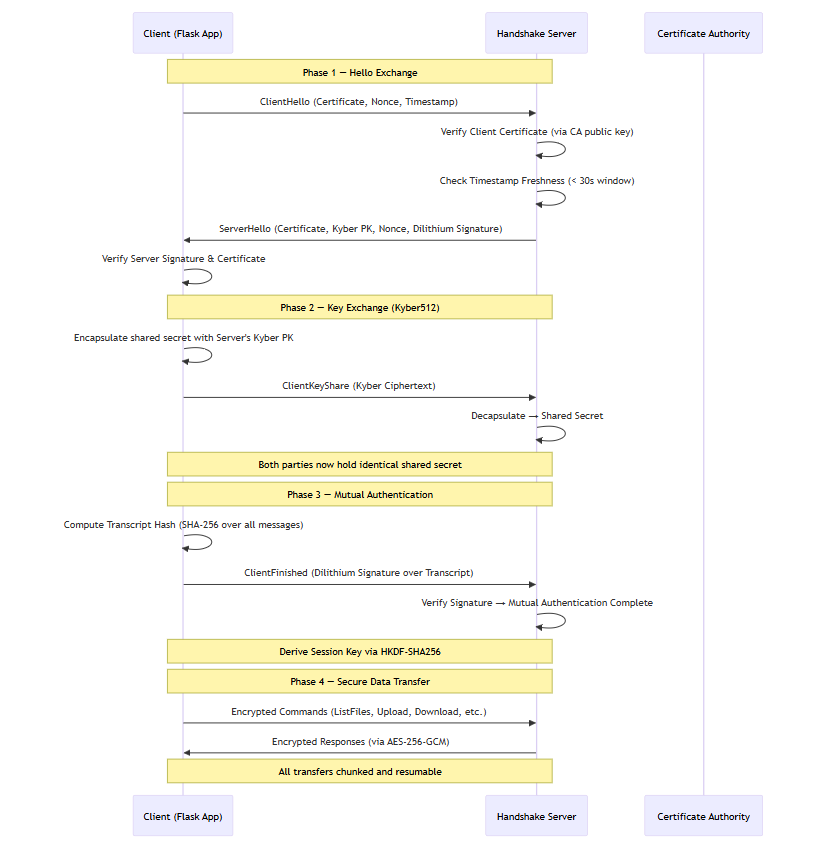
\includegraphics[width=\textwidth]{Figures/PQC_Handshake.png}
    \caption{PQC Handshake Protocol — Four-Phase Mutual Authentication}
    \label{fig:pqc_diagram}
\end{figure}

\subsection{Authentication and Session Flow}

Figure~\ref{fig:auth_flow} details the end-to-end authentication and session management flow, from user login through certificate-based PQC handshake to encrypted session establishment and subsequent file operations.

\begin{figure}[H]
    \centering
    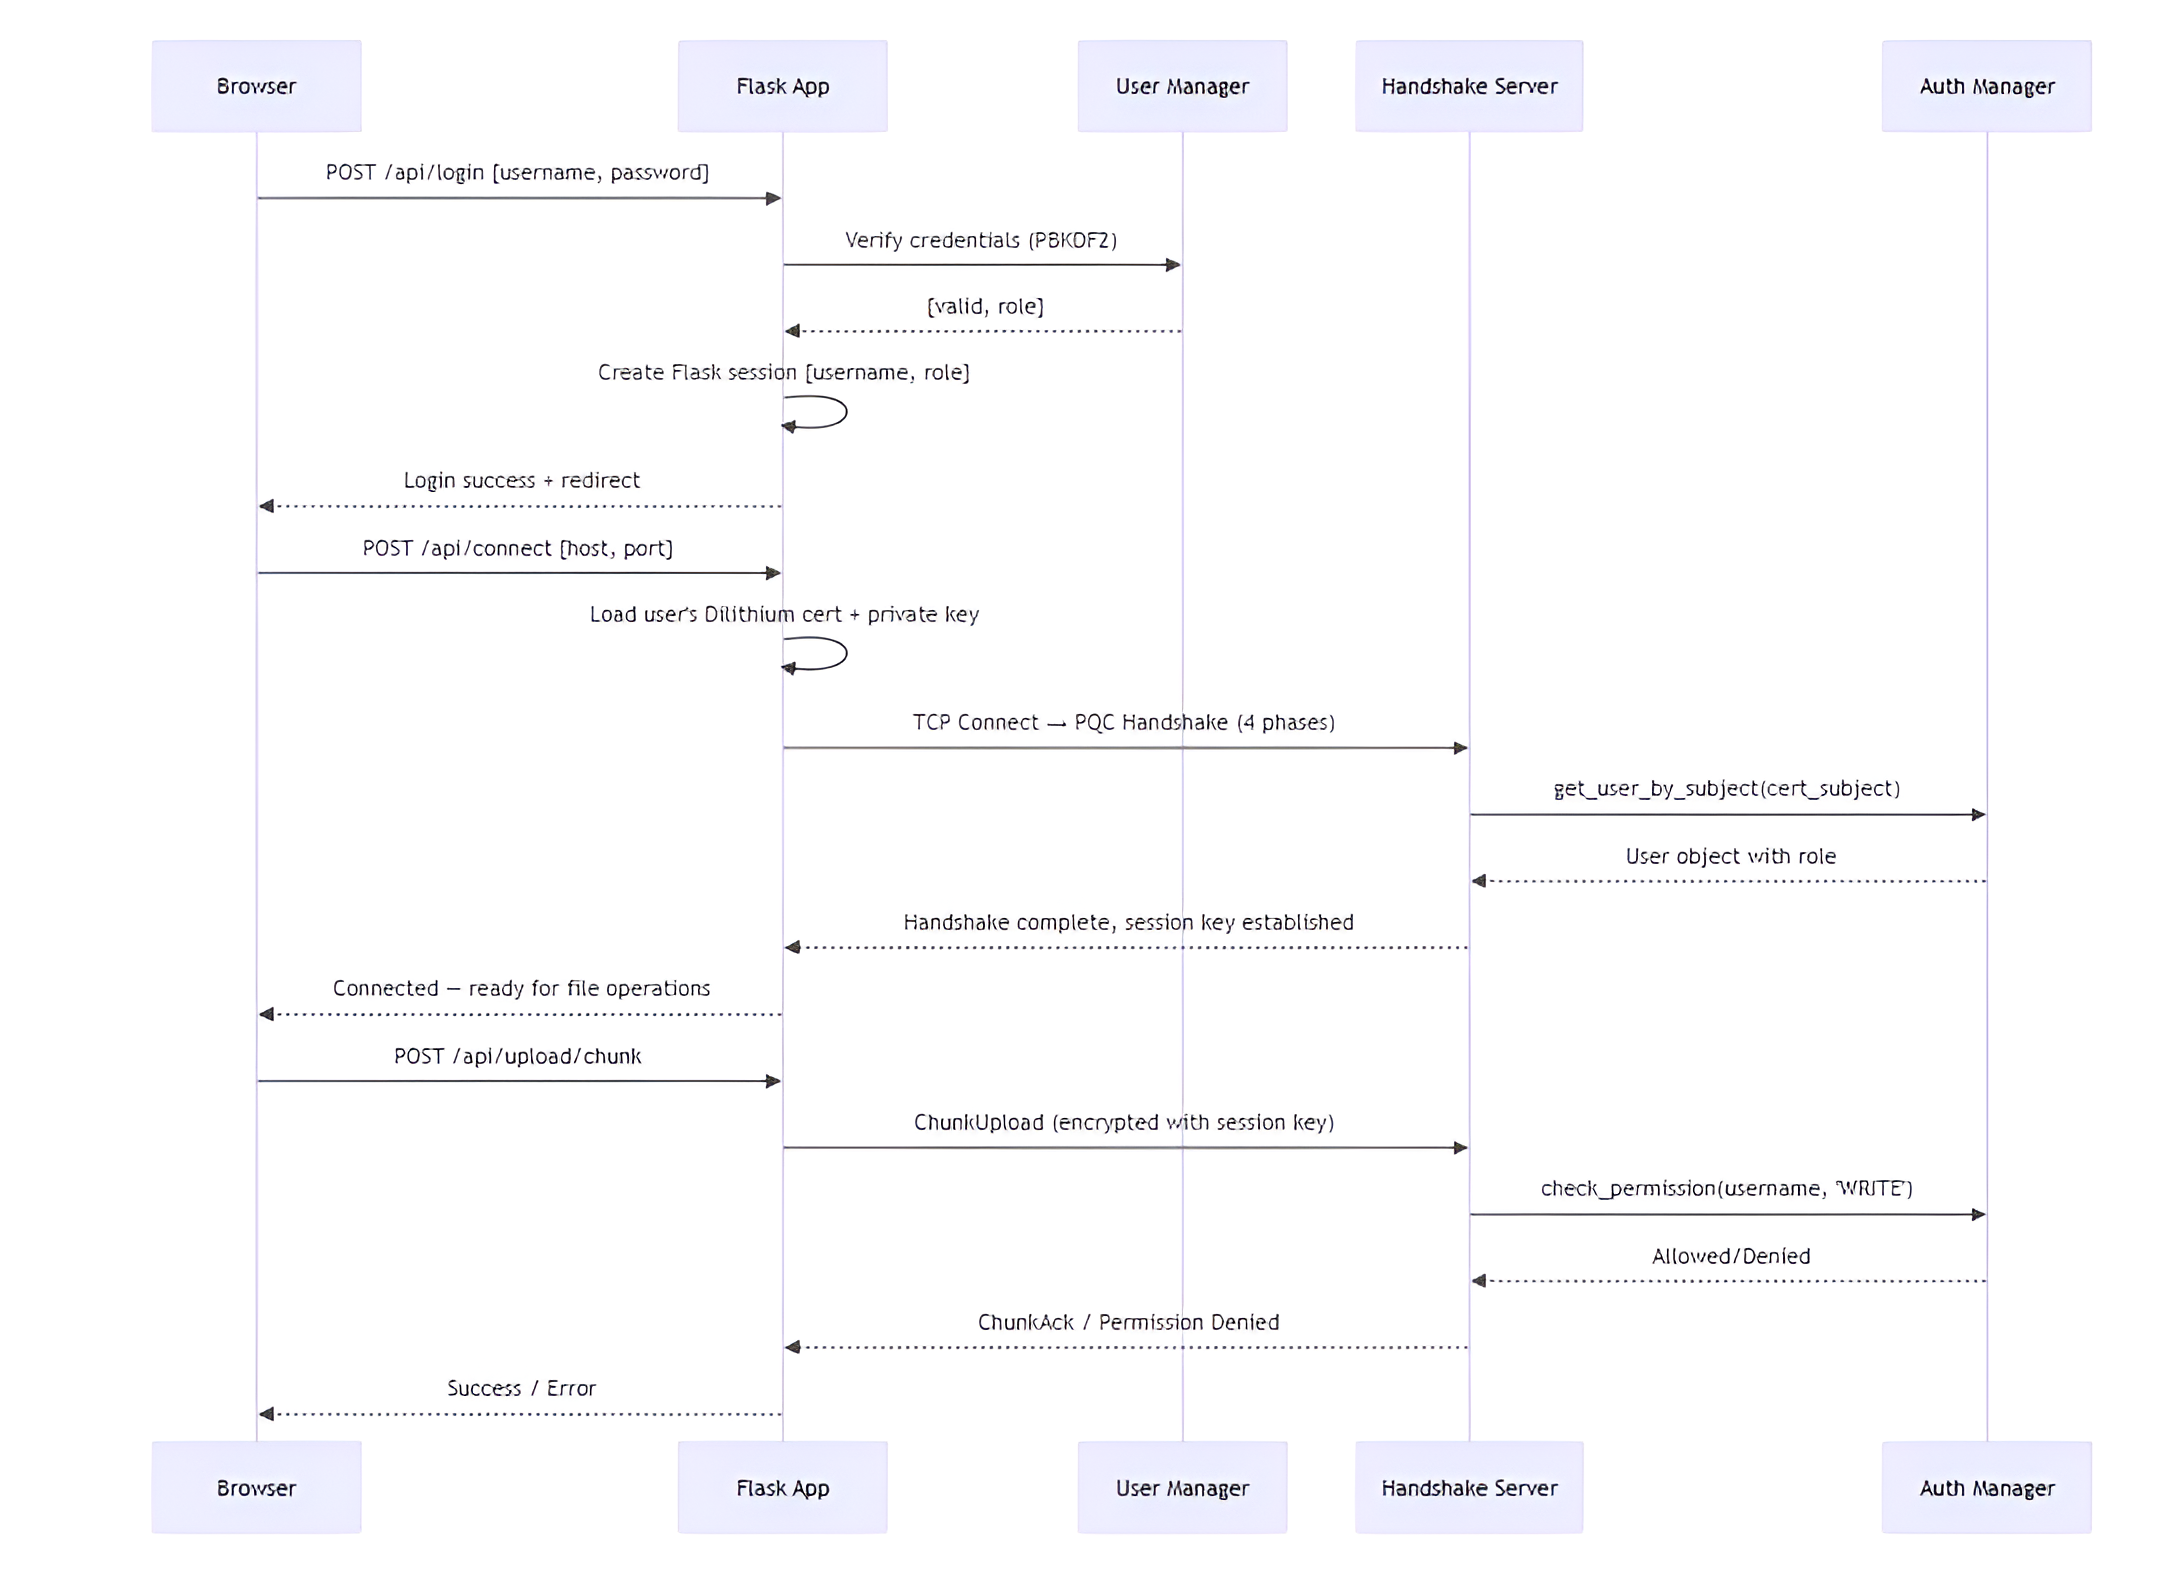
\includegraphics[width=\textwidth]{Figures/Authentication and Session Flow.png}
    \caption{Authentication \& Session Flow — Login to Encrypted File Operations}
    \label{fig:auth_flow}
\end{figure}

\subsection{Role-Based Access Control (RBAC)}

Figure~\ref{fig:rbac_diagram} visualizes the three-tier RBAC model with directory isolation, showing how Administrator, Standard, and Guest roles map to permitted operations and storage boundaries.

\begin{figure}[H]
    \centering
    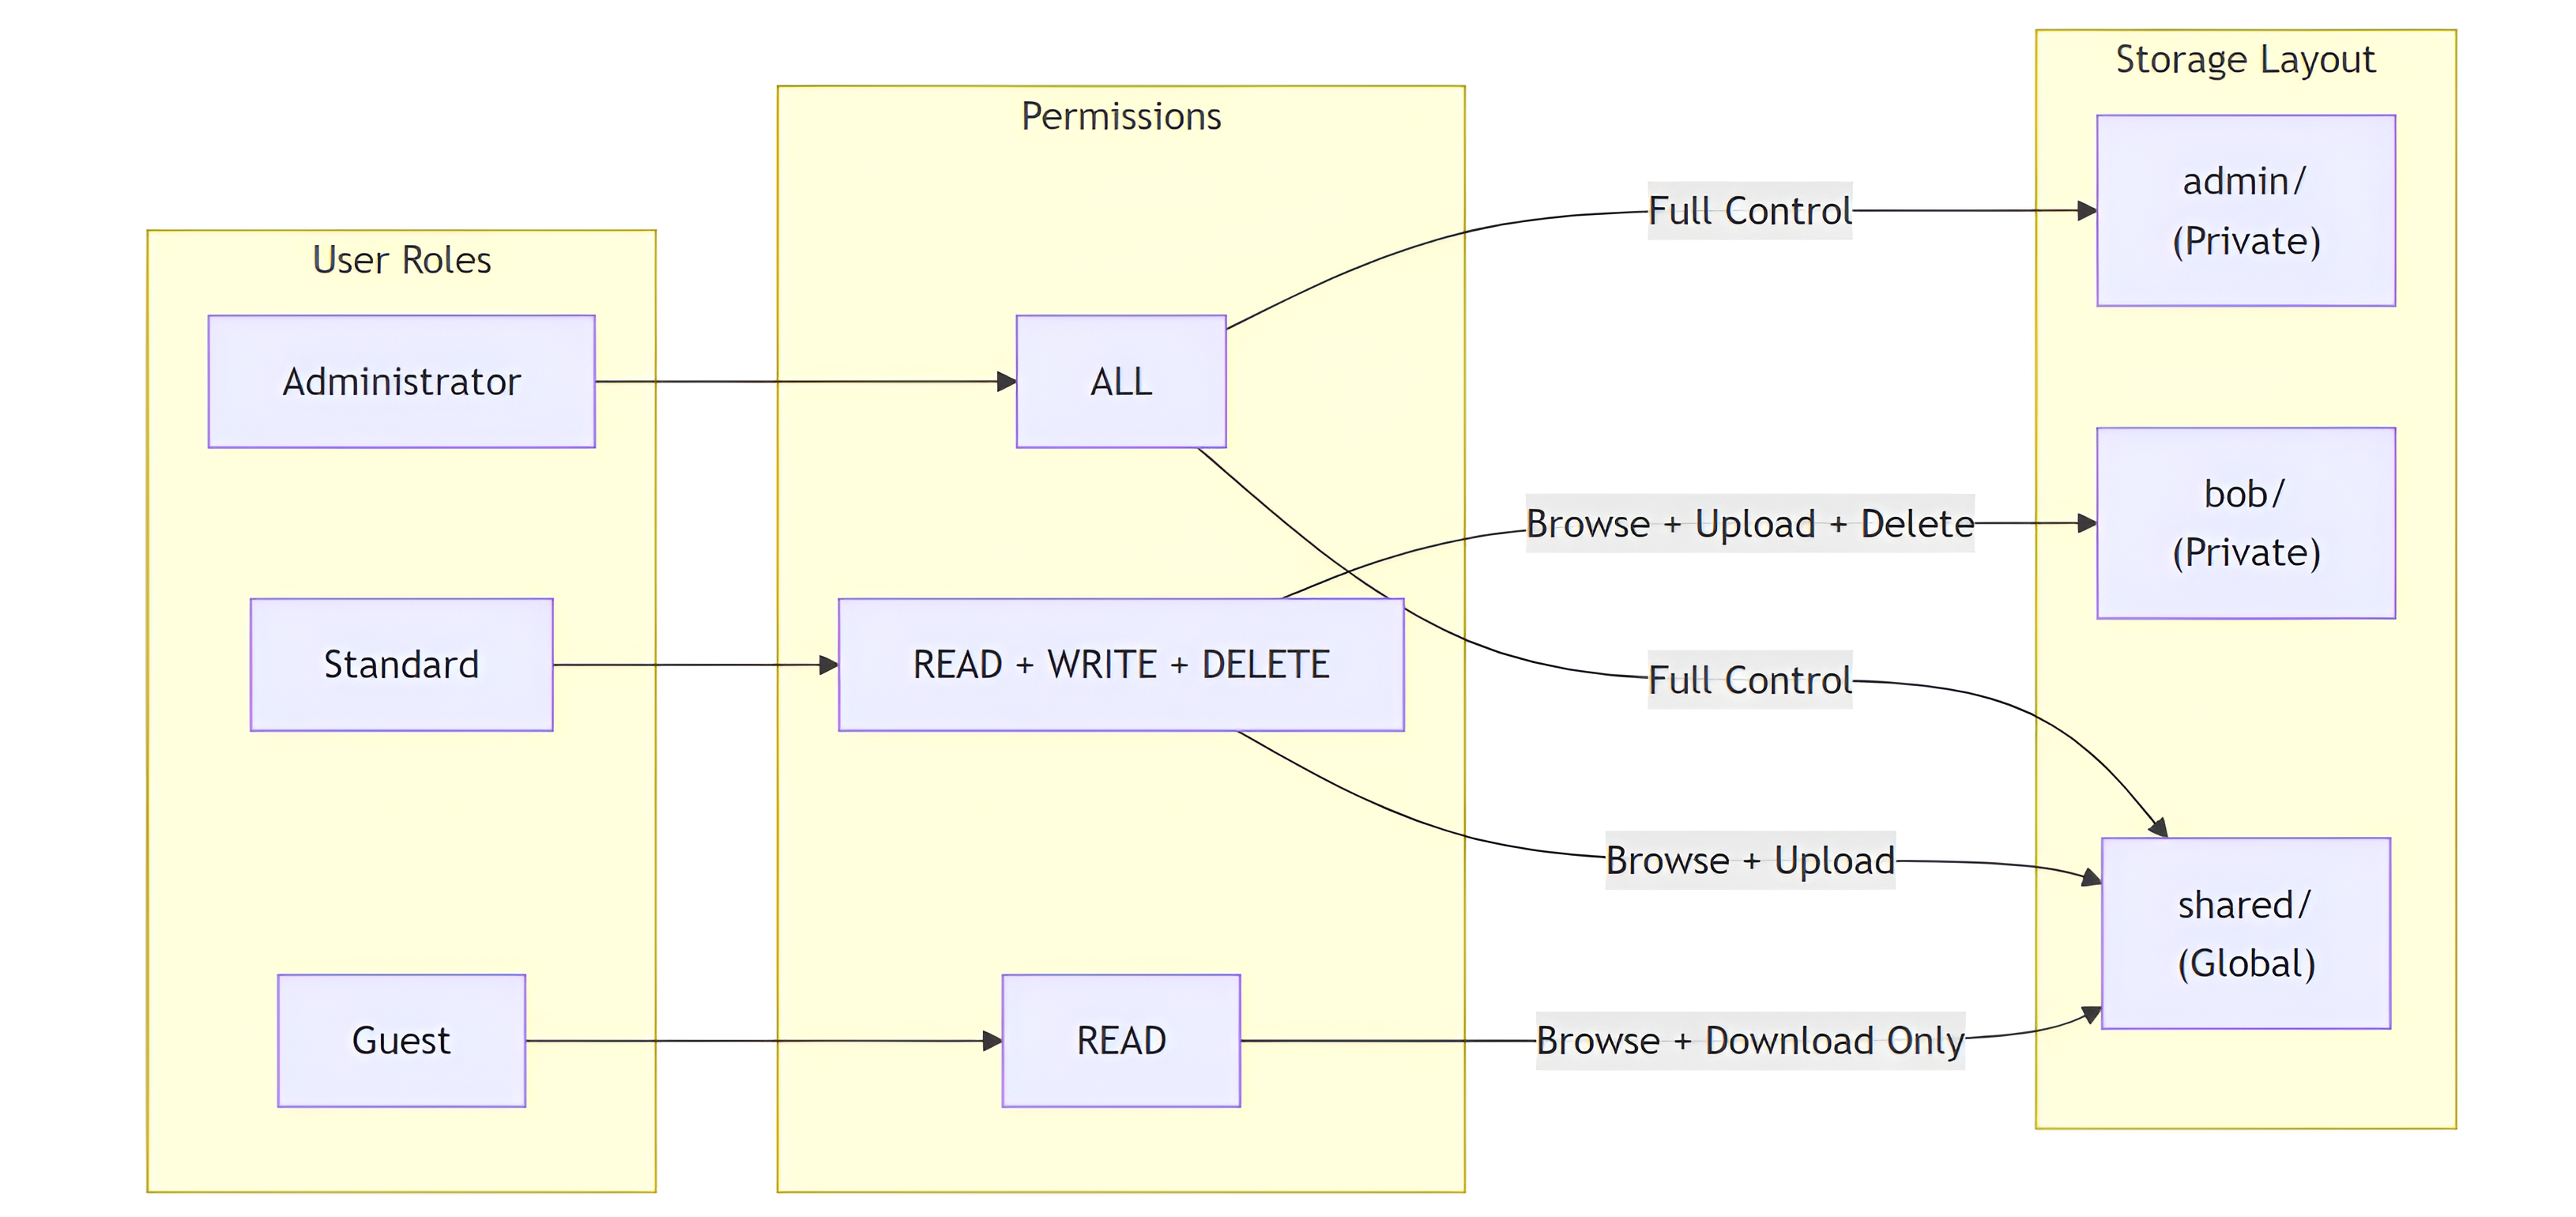
\includegraphics[width=\textwidth]{Figures/RBAC.png}
    \caption{Role-Based Access Control — Permission Model and Directory Isolation}
    \label{fig:rbac_diagram}
\end{figure}

\subsection{Resumable File Transfer Protocol}

Figure~\ref{fig:resume_diagram} depicts the chunked resumable transfer protocol, illustrating chunk processing, state persistence (client-side localStorage and server-side JSON log), and the resume-from-offset mechanism.

\begin{figure}[H]
    \centering
    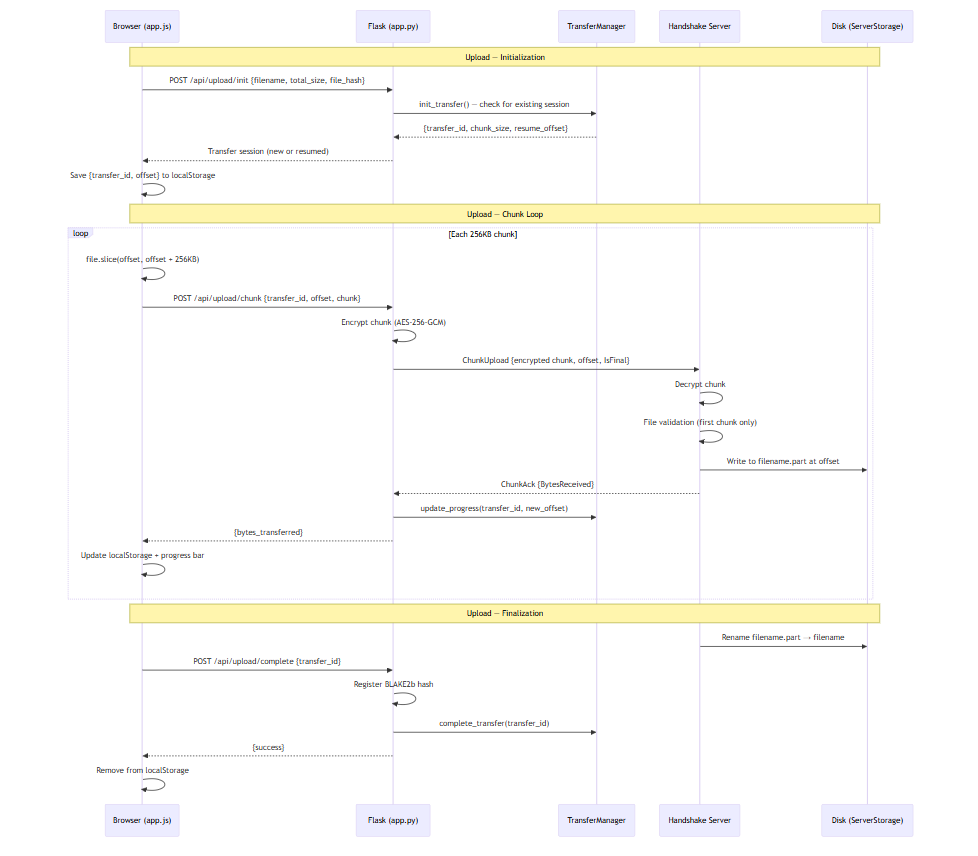
\includegraphics[width=\textwidth]{Figures/Resumable_File_Transfers.png}
    \caption{Resumable File Transfers — Chunked Protocol with State Persistence}
    \label{fig:resume_diagram}
\end{figure}

\section{Testing and Validation}

Testing was been performed to ensure that every module operates securely and efficiently:
\begin{itemize}
\item \textbf{Unit Testing:} Validates individual cryptographic operations (Kyber encapsulation/decapsulation, Dilithium signing/verification, BLAKE2b hashing).
\item \textbf{Integration Testing:} Validates the complete handshake flow between CA, server, and client modules, including certificate generation, mutual authentication, and session key derivation.
\item \textbf{Performance Testing:} Measures handshake latency, file transfer throughput, and chunk processing overhead.
\item \textbf{Security Validation:} Verifies resistance to replay attacks, certificate forgery, man-in-the-middle attacks, and file tampering.
\item \textbf{Hash Phase Testing:} A four-phase testing suite validates the hash infrastructure across registration, verification, tamper detection, and bulk operations.
\end{itemize}

For additional context, refer to Chapter~\ref{chap.2} for the background and Chapter~\ref{chap.3} for related work supporting the design rationale.

\chapter{Contribution}
\lhead{Chapter 5. \emph{Contribution}}
\label{chap.5}

This chapter presents the key contributions of the Quantum Secure File Transfer Protocol (Q-SFTP) project, highlighting the novel aspects and significant technical advancements achieved in the implementation.

\section{Innovations of the Proposed Method}

The novelty of this project lies in the design and implementation of a complete, production-grade post-quantum file transfer system. While prior works have focused on individual cryptographic algorithms or theoretical protocol designs, Q-SFTP uniquely combines the following innovations:

\begin{enumerate}
    \item \textbf{Full PQC Integration:} Complete replacement of classical cryptographic primitives with NIST-standardized algorithms:
    \begin{itemize}
        \item \textbf{CRYSTALS-Kyber512} (FIPS 203 / ML-KEM) for key encapsulation, providing 128-bit post-quantum security.
        \item \textbf{CRYSTALS-Dilithium2} (FIPS 204 / ML-DSA) for digital signatures, providing tamper-proof mutual authentication.
        \item \textbf{AES-256-GCM} for symmetric encryption with authenticated integrity.
    \end{itemize}
    
    \item \textbf{Four-Phase Mutual Authentication:} A novel handshake protocol achieving mutual authentication through certificate exchange, Kyber key encapsulation, transcript hashing, and dual Dilithium signatures — all within four round-trips.
    
    \item \textbf{BLAKE2b-256 Integrity Ecosystem:} Unlike simple checksum approaches, Q-SFTP implements a comprehensive integrity ecosystem with dual-side hash verification (client and server), a persistent hash registry, and a background integrity checker that periodically re-verifies all stored files.
    
    \item \textbf{Chunked Resumable Transfers over PQC Channels:} A chunked transfer protocol that operates within the PQC-encrypted channel, with persistent state tracking on both client (localStorage) and server (JSON log), enabling pause/resume across sessions and connection failures.
    
    \item \textbf{Privacy-Preserving File Storage:} Automatic metadata stripping for images (EXIF), PDFs, and DOCX files before storage, combined with IP anonymization in activity logs using daily rotating salts.
    
    \item \textbf{Lightweight Post-Quantum CA:} A self-contained Certificate Authority built entirely on Dilithium2, without dependency on classical X.509 infrastructure.
\end{enumerate}

\section{Key Technical Contributions}

\subsection{Modular Security Architecture}

The four-tier modular architecture (Client $\rightarrow$ Flask $\rightarrow$ Handshake Server $\rightarrow$ Storage) separates concerns such that cryptographic primitives can be upgraded independently of the application logic. This design anticipates future NIST standard revisions or the adoption of alternative PQC algorithms.

\subsection{Defense-in-Depth File Protection}

Q-SFTP implements multiple layers of file protection:

\begin{table}[H]
    \centering
    \caption{Defense-in-depth layers for file protection}
    \label{tab:defense}
    \begin{tabular}{|l|l|p{7cm}|}
        \hline
        \textbf{Layer} & \textbf{Module} & \textbf{Protection} \\
        \hline
        Transport & Handshake Server & AES-256-GCM encryption with Kyber-derived session keys \\
        \hline
        Validation & FileValidator & Extension blacklisting (17 types) + magic number verification (20+ formats) \\
        \hline
        Integrity & HashVerifier & Dual-side BLAKE2b-256 + persistent registry + periodic background checks \\
        \hline
        Privacy & PrivacyManager & EXIF/PDF/DOCX metadata stripping + IP anonymization \\
        \hline
        Access & AuthManager + RBAC & Three-tier role enforcement + directory isolation \\
        \hline
        Audit & ActivityLogger & Tamper-evident log chain with hash chaining \\
        \hline
    \end{tabular}
\end{table}

\subsection{Production-Ready Web Interface}

Unlike most PQC research prototypes that provide only CLI interfaces, Q-SFTP includes a fully functional web GUI that:
\begin{itemize}
    \item Abstracts all cryptographic complexity behind an intuitive FTP-style interface.
    \item Provides real-time progress bars for chunked transfers with pause/resume controls.
    \item Includes an admin panel for user management, activity log viewing, and integrity monitoring.
    \item Supports dark/light theme switching and responsive design.
\end{itemize}

\section{Novel Findings}

During development and testing, several noteworthy findings emerged:

\begin{itemize}
    \item \textbf{Certificate Size Optimization:} Post-quantum certificates are inherently larger than classical ones (Dilithium2 public keys are 1,312 bytes vs. RSA-2048's 256 bytes). However, the one-time cost during handshake does not significantly impact overall transfer performance.
    
    \item \textbf{BLAKE2b Performance Advantage:} Client-side BLAKE2b computation using the \texttt{blakejs} library proved approximately 3$\times$ faster than SHA-256 via the WebCrypto API for file hashing, confirming its suitability for real-time integrity verification.
    
    \item \textbf{Resumable Transfer Resilience:} Testing demonstrated that chunked transfers with 256 KB chunks and localStorage persistence can reliably survive connection interruptions, browser refreshes, and even system restarts, with minimal overhead ($\approx 0.01\%$ for cryptographic framing).
    
    \item \textbf{Protocol Adaptability:} The modular architecture allowed the complete replacement of the original DH-based key exchange with Kyber512 without modifying any file management or UI code — validating the separation-of-concerns design.
\end{itemize}

\section{Comparison with Existing Solutions}

\begin{table}[H]
    \centering
    \caption{Feature comparison: Q-SFTP vs. existing approaches}
    \label{tab:comparison}
    \begin{tabular}{|l|c|c|c|}
        \hline
        \textbf{Feature} & \textbf{Classical SFTP} & \textbf{Hybrid PQ-TLS} & \textbf{Q-SFTP (Ours)} \\
        \hline
        Quantum-safe KEM & $\times$ & \checkmark & \checkmark \\
        \hline
        Quantum-safe Signatures & $\times$ & Partial & \checkmark \\
        \hline
        Mutual Authentication & \checkmark & \checkmark & \checkmark \\
        \hline
        File Integrity (BLAKE2b) & $\times$ & $\times$ & \checkmark \\
        \hline
        Resumable Transfers & $\times$ & $\times$ & \checkmark \\
        \hline
        Metadata Stripping & $\times$ & $\times$ & \checkmark \\
        \hline
        RBAC + Isolation & Partial & Partial & \checkmark \\
        \hline
        Web GUI & $\times$ & $\times$ & \checkmark \\
        \hline
        Admin Panel & $\times$ & $\times$ & \checkmark \\
        \hline
    \end{tabular}
\end{table}

In total, the contributions of this work go beyond cryptographic algorithm integration to deliver a comprehensive, deployable system with security, usability, and reliability features necessary for practical adoption.

\chapter{Results and Analysis}
\lhead{Chapter 6. \emph{Results and Analysis}}
\label{chap.6}

This chapter presents the results of evaluating the Quantum Secure File Transfer Protocol (Q-SFTP) across multiple dimensions: handshake correctness, cryptographic security, file integrity, transfer performance, and production readiness.

\section{Handshake Verification}

\subsection{Client and Server Handshake Output}

The Q-TLS handshake was tested across localhost and cross-device configurations. Figures~\ref{fig:client_handshake} and~\ref{fig:server_handshake} show the successful execution of the four-phase handshake from client and server perspectives.

\begin{figure}[H]
    \centering
    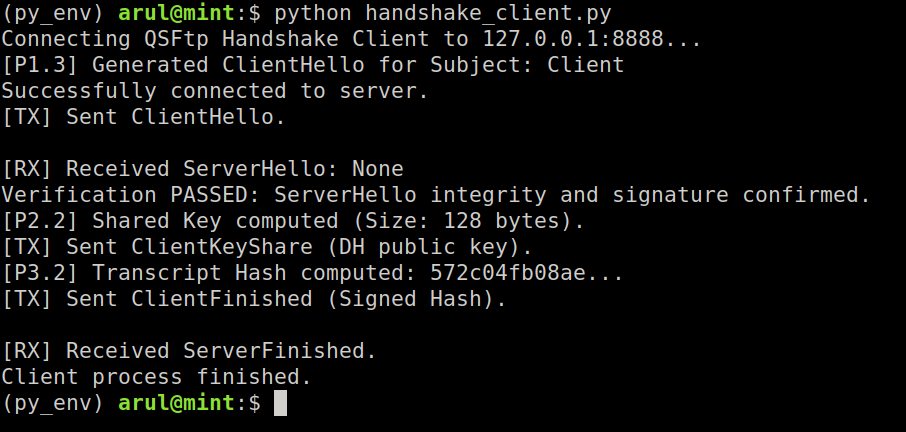
\includegraphics[width=0.9\textwidth]{Figures/client.png}
    \caption{Client-side output of the Q-TLS Handshake showing certificate verification, Kyber512 encapsulation, transcript hash computation, and session key derivation}
    \label{fig:client_handshake}
\end{figure}

\begin{figure}[H]
    \centering
    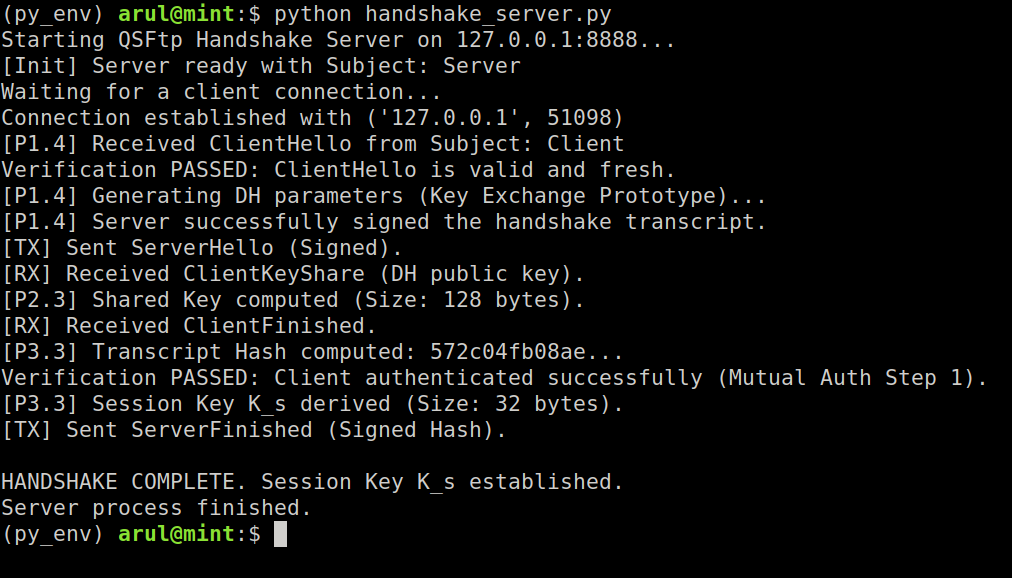
\includegraphics[width=0.9\textwidth]{Figures/server.png}
    \caption{Server-side output of the Q-TLS Handshake showing certificate validation, Kyber512 decapsulation, Dilithium2 signature verification, and session key establishment}
    \label{fig:server_handshake}
\end{figure}

The outputs confirm:
\begin{itemize}
    \item Both endpoints successfully negotiated session keys using Kyber512-based encapsulation.
    \item Mutual authentication was achieved through Dilithium2 signatures on the transcript hash.
    \item Session key derivation via HKDF-SHA256 produced identical 256-bit keys on both sides.
    \item Timestamp validation (30-second window) prevented acceptance of stale messages.
\end{itemize}

\section{Cryptographic Parameter Analysis}

Table~\ref{tab:crypto_params} summarizes the cryptographic parameters and key sizes used in Q-SFTP.

\begin{table}[H]
    \centering
    \caption{Cryptographic parameters and key sizes in Q-SFTP}
    \label{tab:crypto_params}
    \begin{tabular}{|l|c|c|c|c|}
        \hline
        \textbf{Algorithm} & \textbf{Security Level} & \textbf{Public Key} & \textbf{Secret Key} & \textbf{CT / Signature} \\
        \hline
        Kyber512 & NIST Level 1 & 800 B & 1,632 B & 768 B \\
        \hline
        Dilithium2 & NIST Level 2 & 1,312 B & 2,560 B & 2,420 B \\
        \hline
        AES-256-GCM & 128-bit (PQ) & -- & 32 B & +28 B (12 nonce + 16 tag) \\
        \hline
        BLAKE2b-256 & 128-bit (PQ) & -- & -- & 32 B \\
        \hline
    \end{tabular}
\end{table}

\begin{table}[H]
    \centering
    \caption{Dilithium Performance Benchmarks}
    \vspace{2pt}
    \label{tab:dilithium_benchmarks}
    \begin{tabular}{|l|c|c|c|}
        \hline
        \textbf{Operation} & \textbf{Dilithium2} & \textbf{Dilithium3} & \textbf{Dilithium5} \\
        \hline
        KeyGen() & 6 ms & 9 ms & 15 ms \\
        \hline
        Sign() & 27 ms & 46 ms & 58 ms \\
        \hline
        Verify() & 7 ms & 11 ms & 18 ms \\
        \hline
    \end{tabular}
    \vspace{2pt}
    % \small{\textit{\n Hardware: Intel Core i7-9750H CPU}}
\end{table}

\begin{table}[H]
    \centering
    \caption{Kyber Performance Benchmarks}
    \label{tab:kyber_benchmarks}
    \begin{tabular}{|l|c|c|c|c|c|c|}
        \hline
        \textbf{Params} & \textbf{keygen} & \textbf{keygen/s} & \textbf{encap} & \textbf{encap/s} & \textbf{decap} & \textbf{decap/s} \\
        \hline
        Kyber512 & 2.02 ms & 493.99 & 2.84 ms & 352.53 & 4.12 ms & 242.82 \\
        \hline
        Kyber768 & 3.40 ms & 294.13 & 4.38 ms & 228.41 & 6.06 ms & 165.13 \\
        \hline
        Kyber1024 & 5.09 ms & 196.61 & 6.22 ms & 160.72 & 8.29 ms & 120.68 \\
        \hline
    \end{tabular}
    \vspace{2pt}
    % \small{\textit{Hardware: Intel Core i7-9750H CPU}}
\end{table}

\section{Security Testing}

Security testing was performed using automated test scripts and manual verification. The \textbf{pytest} framework was used to validate protocol correctness and cryptographic integrity.

\subsection{Pytest Results for Q-TLS Handshake}

Figure~\ref{fig:pytest_handshake} shows the successful execution of the handshake test suite. All test cases — including certificate exchange, key encapsulation, mutual authentication, and session key derivation — passed.

\begin{figure}[H]
    \centering
    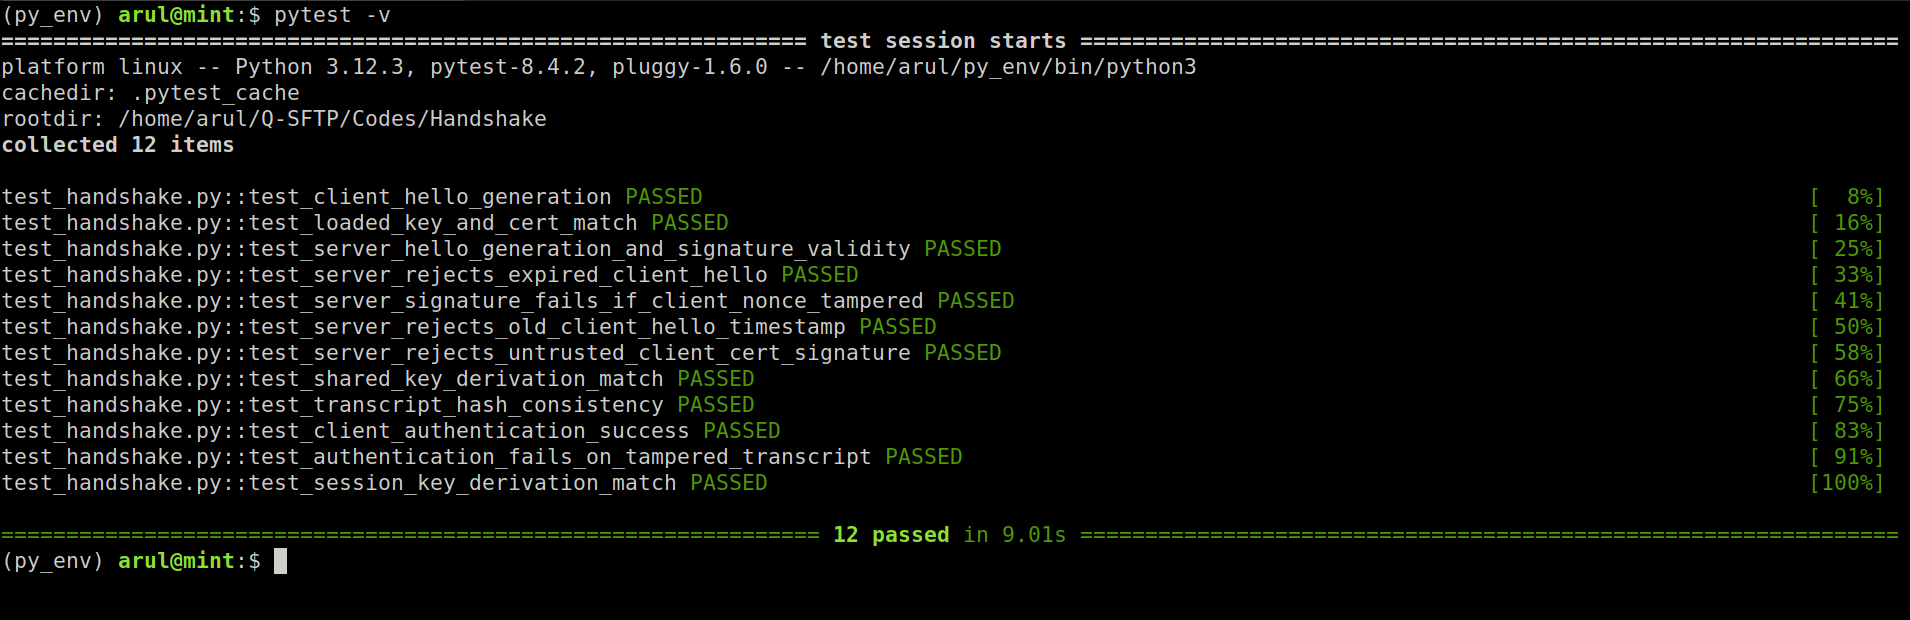
\includegraphics[width=0.9\textwidth]{Figures/pytest_handshake.png}
    \caption{Pytest Results for Q-TLS Handshake Validation}
    \label{fig:pytest_handshake}
\end{figure}

\subsection{CA Tool Testing}

The Certificate Authority module was tested separately to ensure accurate certificate issuance and Dilithium2 signature verification. Figure~\ref{fig:pytest_ca} illustrates the results.

\begin{figure}[H]
    \centering
    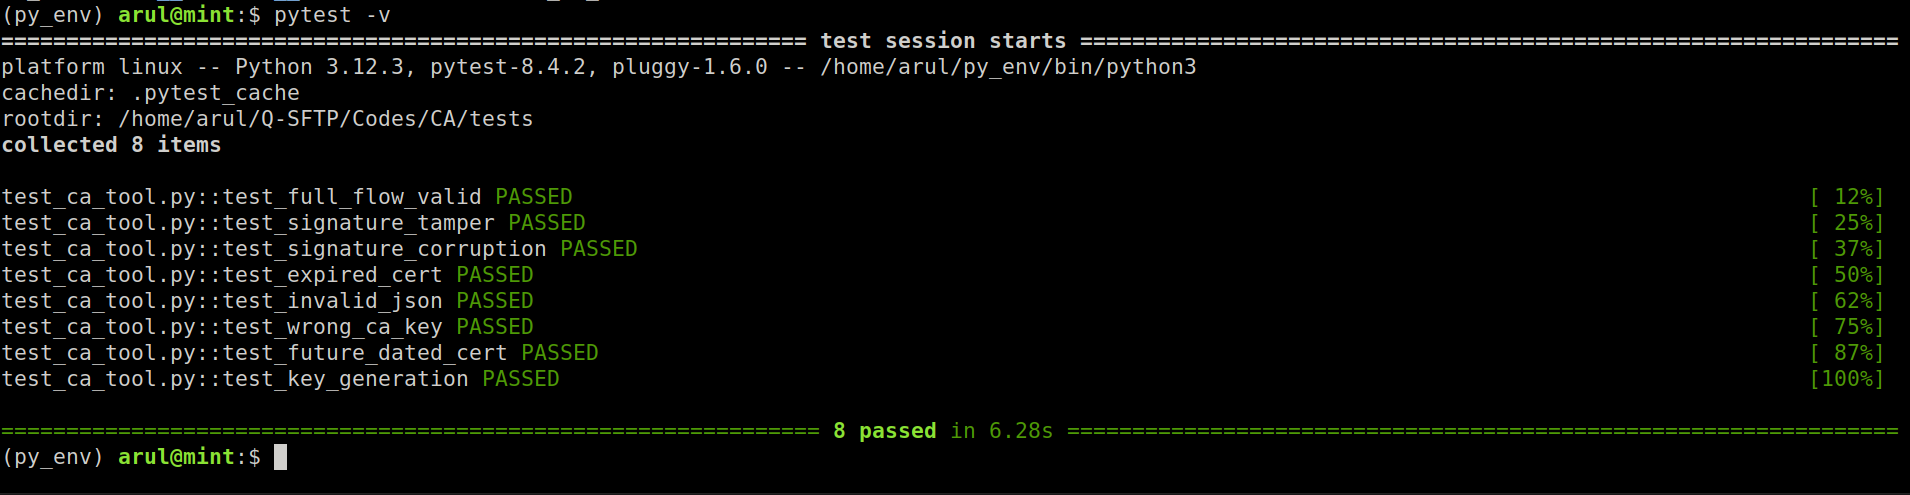
\includegraphics[width=0.9\textwidth]{Figures/pytest_ca.png}
    \caption{Pytest Results for Certificate Authority (CA) Module}
    \label{fig:pytest_ca}
\end{figure}

\subsection{File Integrity Testing (BLAKE2b)}

The BLAKE2b hash verification system was tested in four phases:

\begin{enumerate}
    \item \textbf{Phase 1 — Registration:} Files uploaded via the web interface are automatically hashed with BLAKE2b-256 and registered in \texttt{hash\_registry.json}. All test files were correctly registered with matching client-side and server-side hashes.
    
    \item \textbf{Phase 2 — Verification:} Retrieved files were re-hashed and compared against stored values. All files returned \texttt{VERIFIED} status.
    
    \item \textbf{Phase 3 — Tamper Detection:} Files were manually modified on the server. The integrity checker correctly detected mismatches and returned \texttt{TAMPERED} status with detailed reports.
    
    \item \textbf{Phase 4 — Background Monitoring:} The periodic background checker (running at configurable intervals) correctly identified both verified and tampered files during long-running tests.
\end{enumerate}

\section{Transfer Performance}

\subsection{Chunked Transfer Overhead}

The chunked transfer protocol introduces minimal overhead. For a file of size $F$ bytes with chunk size $C = 256$ KB:
\[
N_{chunks} = \left\lceil \frac{F}{C} \right\rceil
\]

Each chunk incurs an AES-256-GCM overhead of 12 bytes (nonce) + 16 bytes (tag) = 28 bytes, plus JSON message framing. For a 100 MB file:
\begin{itemize}
    \item Total chunks: $N = \lceil 100 \times 1024 \times 1024 / 262144 \rceil = 400$
    \item Cryptographic overhead: $400 \times 28 = 11,200$ bytes ($\approx 0.01\%$)
\end{itemize}

\subsection{Resume Reliability}

Resumable transfers were tested under the following conditions:
\begin{itemize}
    \item \textbf{Connection interruption:} Browser closed mid-upload, then reopened. Transfer resumed from the last confirmed chunk offset.
    \item \textbf{Page refresh:} Browser refreshed during upload. localStorage state enabled seamless resume.
    \item \textbf{Server restart:} Handshake server restarted after partial upload. Server-side \texttt{.part} file and transfer log enabled resume after re-handshake.
\end{itemize}

All three scenarios resulted in successful completion without data loss.

\section{Security Analysis}

\subsection{Quantum Resistance}
\begin{itemize}
    \item The Kyber512 key encapsulation provides IND-CCA2 security under the Module Learning With Errors (MLWE) assumption, which is believed to be hard for both classical and quantum computers.
    \item Dilithium2 provides EUF-CMA (Existential Unforgeability under Chosen Message Attack) security under MLWE and Module-SIS.
    \item AES-256-GCM maintains 128-bit security against Grover's algorithm (quadratic speedup reduces 256-bit to effective 128-bit).
\end{itemize}

\subsection{MITM Resistance}
Mutual authentication through bilateral Dilithium signatures on the transcript hash prevents man-in-the-middle attacks. An attacker would need to forge a Dilithium signature — equivalent to solving MLWE.

\subsection{Replay Attack Prevention}
\begin{itemize}
    \item Random nonces ($N_C$, $N_S$) are incorporated into key derivation.
    \item Timestamp validation rejects messages older than 30 seconds.
    \item Ephemeral Kyber key pairs provide forward secrecy per session.
\end{itemize}

\subsection{Data Integrity}
\begin{itemize}
    \item \textbf{In-transit:} AES-256-GCM authentication tags detect any modification during transmission.
    \item \textbf{At-upload:} Dual-side BLAKE2b hashing detects corruption between client and server.
    \item \textbf{At-rest:} Background integrity checker detects unauthorized server-side modifications.
\end{itemize}

\subsection{Privacy}
\begin{itemize}
    \item Metadata stripping removes identifying information from files before storage.
    \item IP anonymization via daily rotating SHA-256 salt prevents long-term tracking in audit logs.
\end{itemize}

\section{Strengths and Weaknesses}

\subsection{Strengths}
\begin{itemize}
    \item \textbf{Full quantum resistance} using NIST-standardized PQC algorithms.
    \item \textbf{Comprehensive integrity} through BLAKE2b dual-verification and background monitoring.
    \item \textbf{Resumable transfers} with persistent state on both client and server.
    \item \textbf{Privacy preservation} through automatic metadata stripping and IP anonymization.
    \item \textbf{Production-ready web interface} with admin panel and RBAC.
    \item \textbf{Modular architecture} enabling independent cryptographic upgrades.
\end{itemize}

\subsection{Weaknesses}
\begin{itemize}
    \item \textbf{Larger certificates:} PQC keys and signatures are significantly larger than classical equivalents, increasing initial handshake payload.
    \item \textbf{Computational overhead:} Kyber and Dilithium operations consume more CPU cycles than RSA/ECDH for key generation and signing.
    \item \textbf{Single-server architecture:} The current implementation does not support distributed or clustered deployment.
\end{itemize}

The results demonstrate that Q-SFTP achieves its design goals of quantum-safe integrity, confidentiality, and usability without significant performance degradation.

\chapter{Conclusion}
\lhead{Chapter 7. \emph{Conclusion}}
\label{chap.7}

This project has presented the design, implementation, and evaluation of a Quantum Secure File Transfer Protocol (Q-SFTP) that addresses the existential threat posed by quantum computing to classical cryptographic systems. By replacing RSA and Diffie-Hellman with NIST-standardized post-quantum algorithms — CRYSTALS-Kyber512 for key encapsulation and CRYSTALS-Dilithium2 for digital signatures — Q-SFTP ensures long-term data security against both classical and quantum adversaries.

The key achievements of this project are:

\begin{enumerate}
    \item \textbf{Four-Phase PQC Handshake:} A novel Quantum-TLS handshake protocol achieving mutual authentication through Kyber512 key encapsulation, Dilithium2 transcript signatures, and HKDF-SHA256 session key derivation — all within four round-trips.
    
    \item \textbf{Comprehensive File Integrity:} A BLAKE2b-256 dual-verification system with a persistent hash registry and background integrity monitoring, detecting both in-transit corruption and at-rest tampering.
    
    \item \textbf{Resumable Chunked Transfers:} A 256 KB chunked transfer protocol with persistent state tracking on both client (localStorage) and server (JSON log), enabling reliable pause/resume across connection interruptions, browser refreshes, and system restarts.
    
    \item \textbf{Defense-in-Depth Security:} Multiple layers of protection including file type validation (extension blacklisting + magic number verification), automatic metadata stripping (EXIF, PDF, DOCX), IP anonymization in audit logs, and three-tier RBAC with per-user directory isolation.
    
    \item \textbf{Production-Ready Deployment:} A modern web GUI abstracting all cryptographic complexity, an admin panel for user and system management, Docker containerization support, and batch-script local deployment — demonstrating that post-quantum security is achievable without sacrificing usability.
    
    \item \textbf{Lightweight Post-Quantum CA:} A self-contained Certificate Authority built entirely on Dilithium2 signatures, with customized certificate serialization that reduced transmission overhead.
\end{enumerate}

Experimental evaluation confirmed that the system achieves its security goals: resistance to quantum cryptanalysis, man-in-the-middle attacks, replay attacks, and file tampering — while maintaining acceptable performance characteristics. The chunked transfer protocol introduces approximately 0.01\% cryptographic overhead per file, and the PQC handshake completes within practical time bounds.

Despite the larger key sizes inherent to lattice-based cryptography (Dilithium2 public keys are 1,312 bytes vs. RSA-2048's 256 bytes), the one-time handshake cost is amortized over the session lifetime and does not significantly impact file transfer throughput.

In summary, Q-SFTP demonstrates that the migration from classical to post-quantum secure communication is both practical and necessary, and that production-grade systems with comprehensive security features can be built using currently available PQC libraries and standards.
\chapter{Future Work}
\lhead{Chapter 8. \emph{Future Work}}
\label{chap.8}

While Q-SFTP provides a comprehensive post-quantum file transfer solution, several promising directions for future enhancement have been identified:

\begin{itemize}
    \item \textbf{Hybrid Key Exchange:} Combining Kyber512 with X25519 (classical ECDH) in a hybrid KEM would provide defense-in-depth against potential unforeseen weaknesses in lattice-based schemes. This approach aligns with IETF draft recommendations for hybrid post-quantum TLS \cite{chen2022hybridtls}.
    
    \item \textbf{End-to-End File Encryption:} Extending the system with per-file encryption keys derived from user passwords or client-side key pairs, ensuring that even the server operator cannot access file contents (zero-knowledge storage).
    
    \item \textbf{Formal Security Verification:} Applying symbolic model checking tools such as ProVerif or the Tamarin prover to formally verify the Q-TLS handshake protocol's security properties (secrecy, authentication, forward secrecy) against automated adversary models.
    
    \item \textbf{WebSocket Transport:} Migrating the chunked transfer protocol from HTTP polling to WebSocket for reduced latency, bidirectional communication, and server-push capabilities — particularly beneficial for real-time transfer progress updates and large-file downloads.
    
    \item \textbf{Performance Benchmarking:} Systematic evaluation of handshake latency, file transfer throughput, and memory usage across varying network conditions (latency, bandwidth, packet loss), file sizes, and concurrent user loads to establish quantitative performance baselines.
    
    \item \textbf{Multi-Server and Cloud Deployment:} Support for distributed deployment with load balancing, database replication, and shared-nothing architecture for horizontal scalability in enterprise environments.
    
    \item \textbf{Advanced Integrity Features:} Extending the hash registry with version tracking (file history), Merkle tree-based bulk verification for efficient integrity checking of large repositories, and real-time file change notifications.
    
    \item \textbf{Cross-Platform Client:} Developing native desktop clients (Electron or Qt-based) with drag-and-drop support and system tray integration, providing an experience comparable to classical FTP clients like FileZilla.
    
    \item \textbf{Post-Quantum Algorithm Agility:} Implementing a negotiation mechanism in the handshake that allows the client and server to dynamically select from multiple PQC algorithms (e.g., Kyber, NTRU, Classic McEliece) based on security requirements and resource constraints.
    
    \item \textbf{Quantum Key Distribution (QKD) Integration:} As quantum networks mature, exploring the integration of hardware-based QKD for session key establishment as an alternative or supplement to software-based PQC key encapsulation.
\end{itemize}

These enhancements will further strengthen Q-SFTP's position as a practical, scalable, and forward-compatible standard for secure file transfer in the post-quantum era.


%-----------------------------------------------------%
%               Appendix
%-----------------------------------------------------%
\lhead{}
\newpage 
\appendix
\input{Chapters/Appendix}

%-----------------------------------------------------%
%               Plagiarism Report
%-----------------------------------------------------%

\clearpage
\chapter*{Plagiarism Report}
\addcontentsline{toc}{chapter}{Plagiarism Report}

This section includes the plagiarism reports generated for the B.Tech project document. As per academic requirements, two separate reports are provided:

\begin{itemize}
    \item \textbf{With Reference:} The report includes all cited and referenced materials to reflect the actual similarity index in context.
\end{itemize}

The similarity index is within the acceptable limit prescribed by the university's academic policies, indicating that the report maintains academic integrity.

\vspace{0.5cm}

\section*{With Reference}
\begin{figure}[h]
\centering
    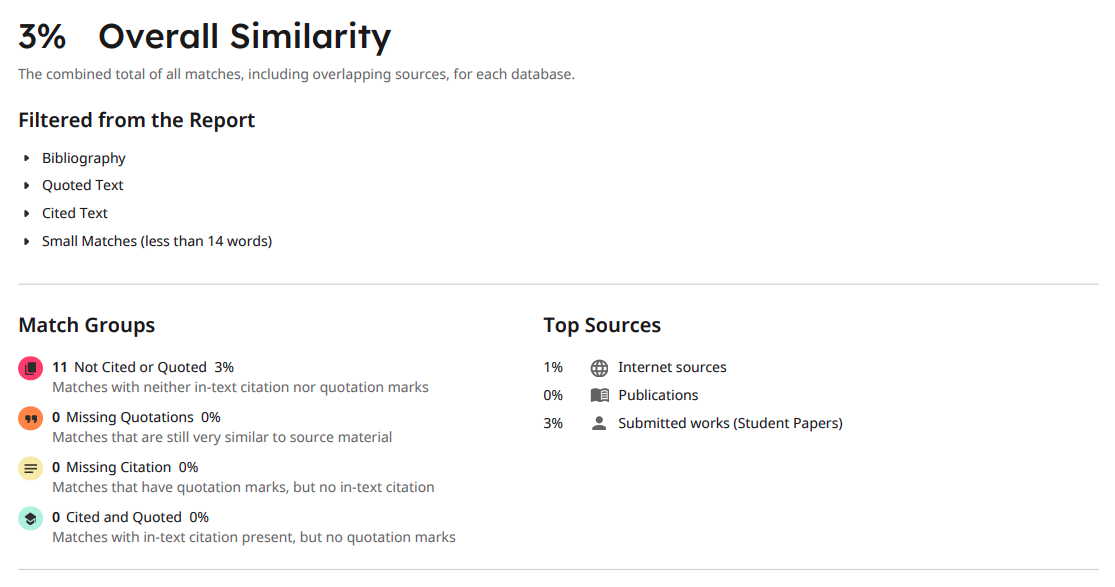
\includegraphics[width=1.1\textwidth]{Figures/turnitin.png}
    \caption{Turnitin Plagiarism Report}
    \label{fig:turnitin_plag_report}
\end{figure}


%-----------------------------------------------------%
%               SDG Alignment
%-----------------------------------------------------%
\clearpage
\chapter*{Contribution to PSOs \& Sustainable Development Goals}
\addcontentsline{toc}{chapter}{Contribution to PSOs \& Sustainable Development Goals}

\noindent\textbf{Title of the Project:} \topic

\noindent\textbf{Project Members Name \& Register Numbers:} \SOneName\ (\SOneRN), \STwoName\ (\STwoRN), 
\SThreeName\ (\SThreeRN), \SFourName\ (\SFourRN)

\noindent\textbf{Guide Name \& Designation:} \gname, \gdes.

\section*{Contribution to PSOs:}
\begin{itemize}
    \item \textbf{PSO 1:}  The project shows a good understanding of the rules for secure communication and post-quantum cryptography. The project builds a Quantum Secure File Transfer Protocol (QSFTP) which transfers files safely even from an adversary who has a quantum computer. In the project, the system encrypts and exchanges keys in a way that a computer using quantum mechanics does not pose a threat to the safety of transferred data. By studying in depth potential quantum-based attack scenarios and countermeasures, the project demonstrates an ability to foresee future security threats and design a system prepared for future security.
    
    \item \textbf{PSO 2:}  The project uses cryptographic techniques and standard security practices to design a practical and efficient file transfer protocol. The project uses quantum-safe algorithms like Kyber for key exchange and Dilithium for digital signatures to protect files from an adversary with a quantum computer. The project’s secure session establishment, file integrity check, and hybrid encryption are both powerful security measures and practical design choices. The project demonstrates an ability to design innovative cybersecurity solutions that follow global standards and are practical for real-world use.
\end{itemize}


\section*{Contribution to SDGs:}
\vspace{1em}

\begin{center}
\renewcommand{\arraystretch}{1.5}
\begin{tabular}{| m{3cm} | m{8cm} |}
    \hline
    \textbf{SDG } & \textbf{Contribution } \\
    \hline
    4. Quality Education & Promotes research and learning in emerging technologies like quantum cryptography and secure communication systems. \\
    \hline
    9. Industry, Innovation and Infrastructure & Develops innovative, quantum-resistant infrastructure for secure data transfer, strengthening digital resilience. \\
    \hline
    16. Peace, Justice and Strong Institutions & Enhances trust, transparency, and data integrity in digital systems, supporting secure and accountable institutions. \\
    \hline
\end{tabular}
\end{center}

\vspace{2em}

\begin{center}
\begin{minipage}{0.3\textwidth}
    \centering
    
\includegraphics[width=0.8\linewidth]{Figures/SDG/G4.png} \\
    \small \textbf{SDG 4}
\end{minipage}
\hspace{1em}
\begin{minipage}{0.3\textwidth}
    \centering
    
\includegraphics[width=0.8\linewidth]{Figures/SDG/G9.png} \\
    \small \textbf{SDG 9}
\end{minipage}
\hspace{1em}
\begin{minipage}{0.3\textwidth}
    \centering
    
\includegraphics[width=0.8\linewidth]{Figures/SDG/G16.png} \\
    \small \textbf{SDG 16}
\end{minipage}
\end{center}

%-----------------------------------------------------%
%               End of Document
%-----------------------------------------------------%
\bibliographystyle{ieeetr}   % or plain, alpha, apalike etc.
\bibliography{references}
\end{document}
